\documentclass[12pt,oneside]{sotsuken_paper}

% タイトル
\title{超低重心6輪独立懸架ローバーの画像情報による自律走行}
\author{佐々井翔也・戸澗健・畠中和久}

\begin{document}
% 行間
\setlength{\baselineskip}{9truemm}

%文字間
\kanjiskip=.53zw plus 3pt minus 3pt
\xkanjiskip=.53zw plus 3pt minus 3pt

% 目次
\tableofcontents
%\newpage

% 本文

\chapter{緒言}
\section{研究の背景}

\subsection{安定性の改善}
前年度,つくばチャレンジで使用したロボットの重心が高かったため,凸凹道やコンクリートなどでロボットが傾きそのまま転倒する恐れがあった.
そのため,前年度の問題点を元に転倒しても走行可能なロボットの開発を試みた.だが,今年度のつくばチャレンジに参加するにあたり,ロボットの高さ制限を満たし,転倒しても走行可能な機構の開発ができなかった.
よって今回はロボットの走破性を高めることで,転倒しにくいロボットの開発を行った.
\subsection{自己位置の推定}
ロボットが自律走行を行うためには,自身の位置を推定する必要がある.
その手段としてローカルマップをグローバルマップに変換する方法が主流である.
これはロボットが何らかの方法で周辺の情報を得る必要があり,一般的に測域センサや地磁気センサが用いられることが多い.
また,近年はカメラを用いた信号認識など視覚情報を用いた研究が活発である.
そこで今回は低コストで省スペース化が期待できる単眼カメラを用いることにした.
\subsection{三角測量とカメラの移動量}
ローカルマップを生成するために周囲との位置関係を求める必要がある.
カメラでは対象物を写した2枚の画像とそれらの画像間距離から三角測量の原理を用いることで対象物からカメラまでの距離を計測することができる.
この原理を用いるためには,カメラの姿勢と移動量が既知の値の必要があり,それらを求めなければならない.



\section{研究の目的}
今年度は走破性の向上を考え,前年度の改善案として低重心化とそれを補佐する懸架装置に注目し,”超低重心6輪独立懸架ローバー”を開発する.またカメラの移動量をモーションセンサから得られる位置情報によって取得し,三角測量を行う.これを複数回行い,得られたデータをマップとする.

\section{論文の構成}
1章では研究背景を中心に本論文で述べる内容を簡略化して示す.2章では我々が参加したつくばチャレンジについて概要を述べる.3章ではつくばチャレンジに参加したロボットの概要について示す.4章では3次元測量を行う実際の手順について述べる.5章では4章で述べた手順でマップを作成した結果について述べる.最後に6章で本論文のまとめを述べる.
\chapter{つくばチャレンジについて} 
%\section{つくばチャレンジの概要} 
\section{つくばチャレンジの概要} 
今年度参加したつくばチャレンジについて説明する.つくばチャレンジとは茨城県南部に位置するつくば市の屋外で行こなわれるロボット実験である.これは人間とロボットの共存する社会の実現のための先端的技術への挑戦が狙いである.人間とロボットの共存を目的とするため,ロボットには以下のことが求められる. 
\begin{enumerate} 
 \item そこにいる人間が安全であること 
\item そこにいる人間に危害を加えないこと.またそのように取られる不安感を与えないこと 
 \item 環境内に存在するものに手を加えないこと.また環境景観を損なわない外観であること 
\item 環境内に存在するものの邪魔にならないこと.また,環境内の運動を妨害しないこと 
\end{enumerate} 
これらの項目が満たされていなければつくばチャレンジでは走行を行うことができない.また,つくばチャレンジではその走行に対して課題が与えられる.以下につくばチャレンジのコースを図\ref{fig:tizu}として示す(つくばチャレンジ2016の課題より参照). 

\begin{figure}[htp] 
 \begin{center} 
  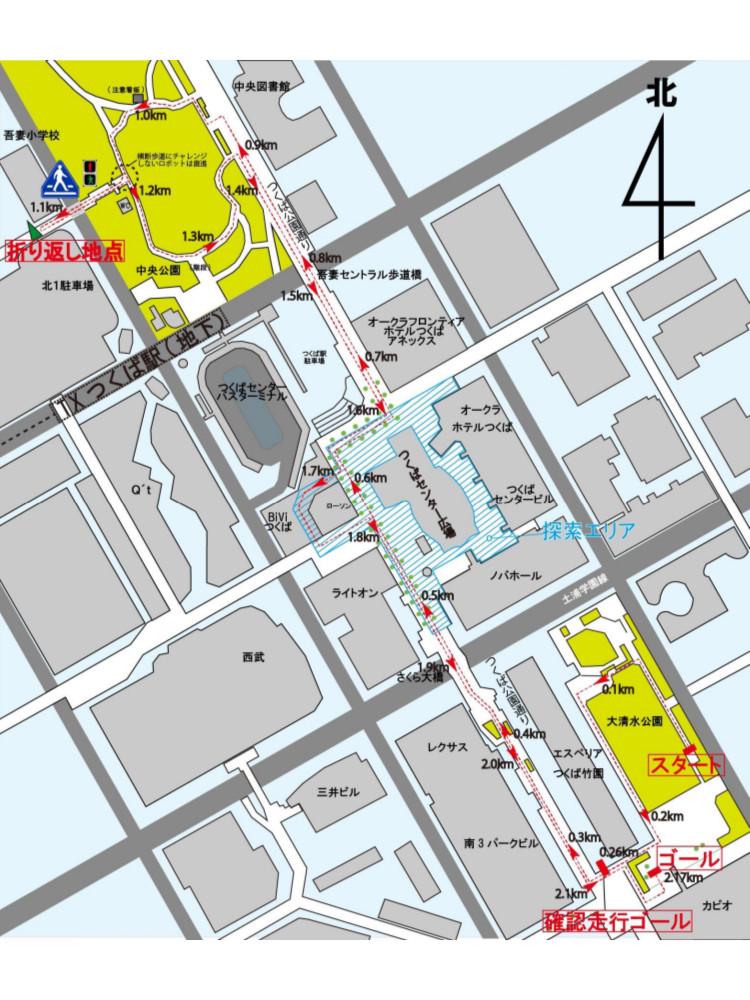
\includegraphics[width=100mm]{img/hard/tizu.jpg} 
  \caption{つくばチャレンジコース図} 
  \label{fig:tizu}%ここに文章中で使用する名前を指定する 
 \end{center} 
\end{figure} 

\section{今年の課題} 
今年度のつくばチャレンジの課題について説明する.全体のコース,コース環境,そしてロボットに必要な機能をそれぞれ述べる.またロボットは歩道橋等を走行するが,その場合原則として端より1m以上離れての走行とされる. 
\subsection{全体のコース} 
本コースのスタート地点は図\ref{fig:tizu}の右下に位置するつくば市大清水公園東側の歩道をスタート点とし,公園内を反時計回りに周回する.コースは大清水公園から遊歩道へと進み,更に北上してつくばセンター広場へと出る.この広場の東側を探索エリアと呼ぶ.センター広場から北上し,途中左折して中央公園に入り,公園内を反時計回りに周回する.中央公園内の周回途中で,一旦右折して信号機付の横断歩道を渡る.そして北1駐車場脇で折り返し,再度横断歩道を渡り中央公園に戻る.中央公園を周回したあと,再度つくば公園通りの遊歩道に戻り,つくばセンター広場に向かって南下する.センター広場では,西側にあるBiViつくば(つくばバスターミナルビル)の2階の自動扉を通り,その中を通り抜ける.そのまま遊歩道を南下大清水公園に戻る.大清水公園入口のつくばカピオ前がゴールである. 

\subsection{コース環境} 
本大会のコースはつくば市民が日頃生活をしている生活環境である.したがって日常のように人や自転車が通行している.つくばチャレンジでは危険防止のため安全責任者を各チーム内から定め,ロボットの走行時には通行人や見物人に注意を呼びかける. 


ロボットの走行エリアと市民の歩く領域は区別されない.天候は当日の天候状況によるが,小雨程度であれば滞り無く開催される.また路面や環境の状況(落ち葉,水たまりなど)も前日やそれ以前の天候,または社会的条件(お祭りなど)に大きく影響を受ける. 


ロボットは環境内にもともと存在する街路樹や縁石柵あるいは建物を走行のガイドとして用いるのは自由であるが,ロボットの走行の為に新しくガイドとなるものを設置することや,環境を改変することは許されない. 

\subsection{ロボットに必要な機能} 
つくばチャレンジは人間が暮らす環境で行われる.人間は多少の凸凹や路面のひび割れ,フレーチングの溝などの障害は問題なく歩行できる.だが,ロボットは人間のようにフレキシブルではない,段差で転んだり溝にハマることが大いに考えられる.よって走行の際に必要なロボットの機能として悪路が走行できる,溝に嵌っても自力で這い上がることができる等路面走行に対してフレキシブルに対応することが求められる. 



\chapter{システムの全体像} 
%この章では3.1から3.3でロボットの全体像, 3.4で前半にメカ,後半に電気設計を記し, 3.5から使用したソフトウェアについて述べていく. 
\section{ロボット構成}
\subsection{ロボットの構成} 
今年度のロボットに搭載したセンサを以下の表\ref{tab:op}に示す. 

\begin{table}[h] 
  \begin{center} 
    \caption{ハードウェアの構成} 
    \small 
  \scalebox{0.85}{ 
  \begin{tabular}{|c|c|} \hline 
    構成要素 & メーカ・型番・スペックなど \\ \hline 
    Mian PC & NVIDIA JETSON TK1 \\ \hline 
    OS & Ubuntu 14.04 LTS \\ \hline 
    camera & Panasonic HX-A1H \\ \hline 
    Buttery & KyPOM KT5100 4S 35C \\ \hline 
    Motor & MABUCHI MOTOR RS-555VC-5524 \\ \hline 
    Motion Sensor & 東京航空計器株式会社 CSM-MG100\\ \hline 

  \end{tabular} 
  } 
    \label{tab:op} 
  \end{center} 
\end{table} 

\subsection{ロボットの外観} 
以下の図\ref{fig:gaikan}にロボットの外観を示す.また,車体の仕様を表\ref{tab:siyou}に示す 

\begin{figure}[htp] 
 \begin{center} 
  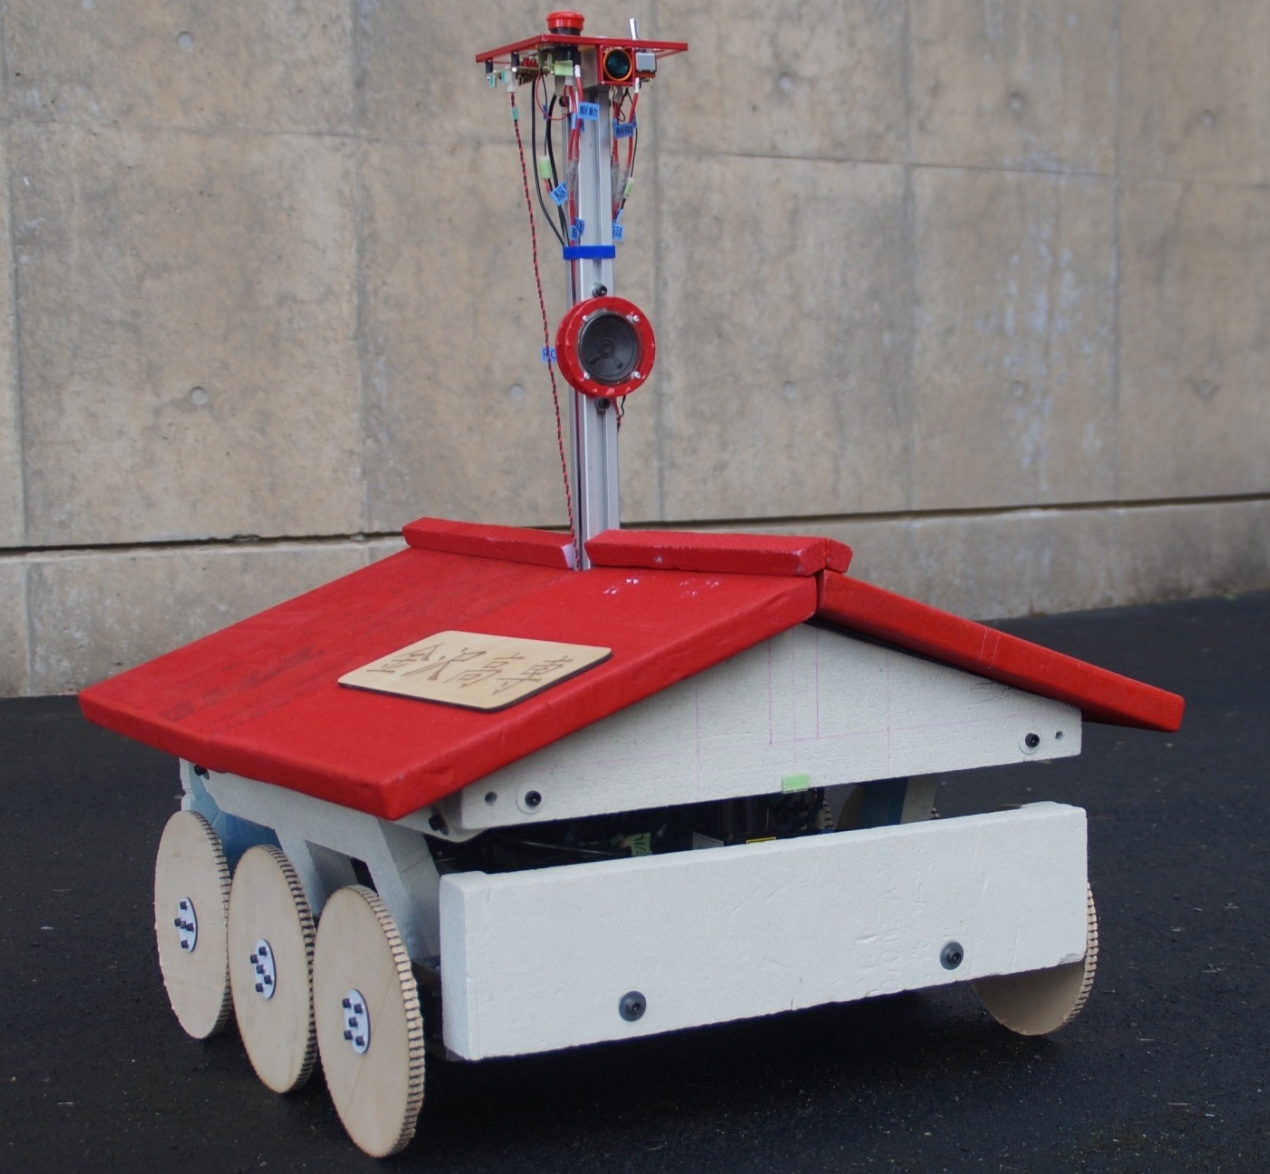
\includegraphics[width=100mm]{img/hard/gaikan.jpg} 
  \caption{ロボットの外観図} 
  \label{fig:gaikan}%ここに文章中で使用する名前を指定する 
 \end{center} 
\end{figure} 

\begin{table}[htp] 
  \begin{center} 
    \caption{車体の仕様} 
  \begin{tabular}{|l|l|l|l|l|l|l|l|} \hline 
全高 & 72[cm] \\  \hline 
全長 & 58[cm] \\ \hline 
車幅 & 61[cm] \\ \hline 
重量 & 20.6[kg] \\ \hline 
駆動形式 & 6車輪2輪駆動 \\ \hline 
タイヤ径 & 直径19[cm] \\ \hline 
使用モータ &  MABUCHI MOTOR RS-555VC-5524\\ \hline 
最大速度 & 4[km/h] \\ \hline 
  \end{tabular} 
    \label{tab:siyou} 
  \end{center} 
\end{table} 



\subsection{システムの構成} 
ロボットのシステム構成を図\ref{fig:sisutemu}に示す.NVIDIA JETSON TK1をUSBハブに接続し,そこから各センサ類に接続する.得られたデータはUSBハブを介してNVIDIA JETSON TK1に送信され,モータ類に指令を与える. 
\begin{figure}[htp] 
 \begin{center} 
  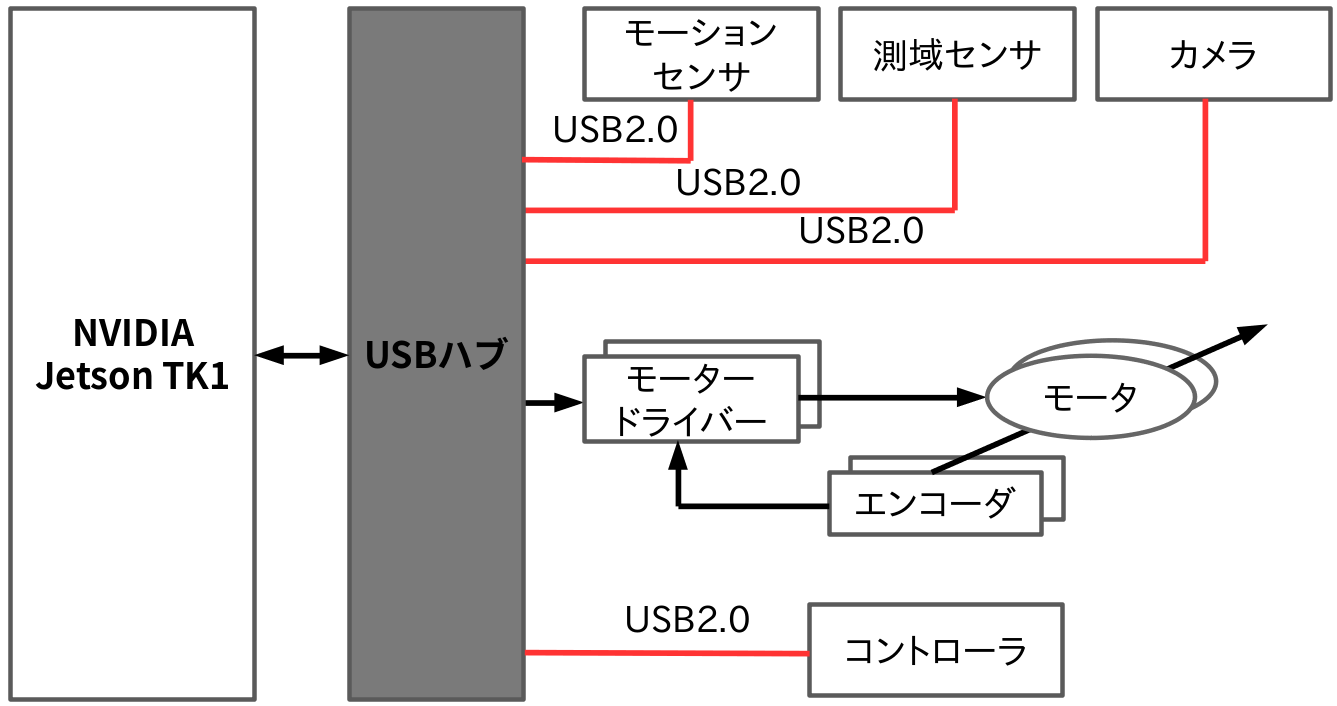
\includegraphics[width=100mm]{img/hard/sisutemu.png} 
  \caption{システム構成} 
  \label{fig:sisutemu}%ここに文章中で使用する名前を指定する 
 \end{center} 
\end{figure} 

\section{機械設計} 

\subsection{ハードウェア開発の狙い} 
サスペンションを内蔵するハードウェアを制作する.つくばチャレンジ2016では走破性向上を目的として低重心を目標としているため,ハードウェアの全高を小さく設計することでその目標に尽くす.また今回のロボットの超低重心を実現するための数値を表\ref{tab:joken} に示す 

\begin{table}[htp] 
  \begin{center} 
    \caption{目標数値} 
  \begin{tabular}{|c|c|c|c|} \hline 
横幅 & 600mm以内  \\  \hline 
長さ & 1000mm以内\\ \hline 
高さ & 150mm以内 \\ \hline 
    乗り越える段差 & およそ30mm  \\ \hline 
  \end{tabular} 
    \label{tab:joken} 
  \end{center} 
\end{table} 

\subsection{サスペンションの概要} 
製作するロボットはある程度の段差を超えるための上下できる機構が必要である.よって近年最も身近な上下機構を持つ機械として,車に利用されるサスペンションを参考にした.図\ref{fig:doublewish}に示すダブルウィッシュボーン式サスペンションは上下のアームとショックアブソーバ,ばねからなるもので,レーシングカーに多く使用されている.図\ref{fig:strat}に示すストラット式サスペンションと呼ばれるものはショックアブソーバとサスペンションを一体化したものをアッパーアームにしたもので,近年の車やミニ四駆などに使用されている.両方とも独立懸架で安定性や利便性に置いてはストラット式が大きく優るが,今回はコンパクトに構成することも必要なため,もともと上下アームで囲われているスペースを活かせることができそうなダブルウィッシュボーン式サスペンションを基礎として開発する. 

\begin{figure}[htp] 
 \begin{center} 
  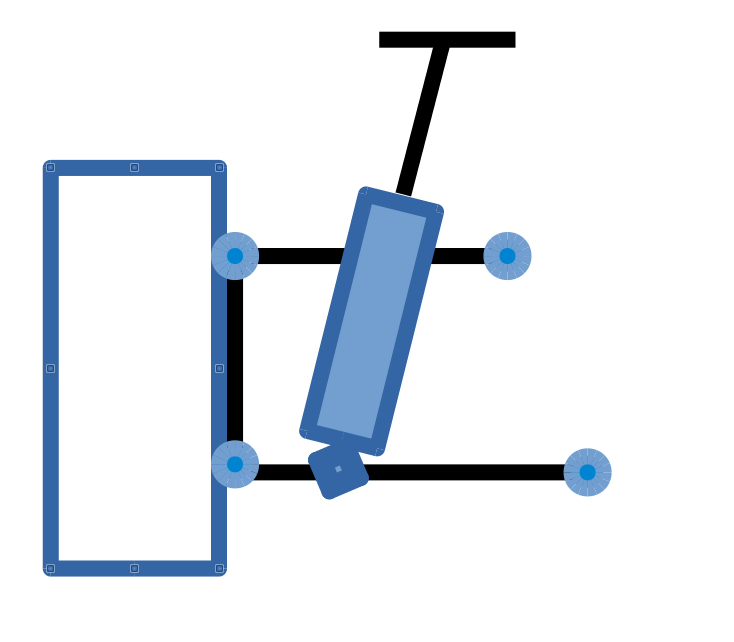
\includegraphics[width=50mm]{img/hard/fig1.png} 
  \caption{ダブルウィッシュボーン式サスペンション} 
  \label{fig:doublewish}%ここに文章中で使用する名前を指定する 
 \end{center} 
\end{figure} 

\begin{figure}[htp] 
 \begin{center} 
  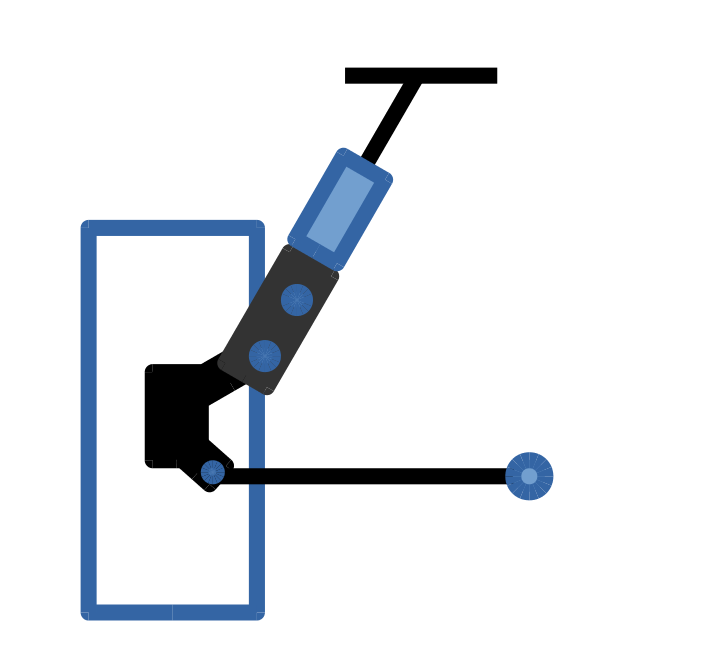
\includegraphics[width=40mm]{img/hard/fig2.png} 
  \caption{ストラット式サスペンション} 
  \label{fig:strat}%ここに文章中で使用する名前を指定する 
 \end{center} 
\end{figure} 

\subsection{メカの概要} 

製作する”超低重心6輪独立懸架ローバー”(以下6輪ローバ)は図\ref{fig:rokurin}に示すとおり低重心であるがゆえにロボットそのものが平たく大きい物になる.そのままではメンテナンス性にかける他,運搬時に非常に不便なため,モータを持つドライブモジュール(以下Dモジュール)と指示塔であるコントロールモジュール(以下Cモジュール)に分解できるようにハードウェアを設計し,分解から組み立てを容易とするようにした.つまり2つのDモジュールと1つのCモジュールからなる1つのハードウェアである. 

\begin{figure}[htp] 
 \begin{center} 
  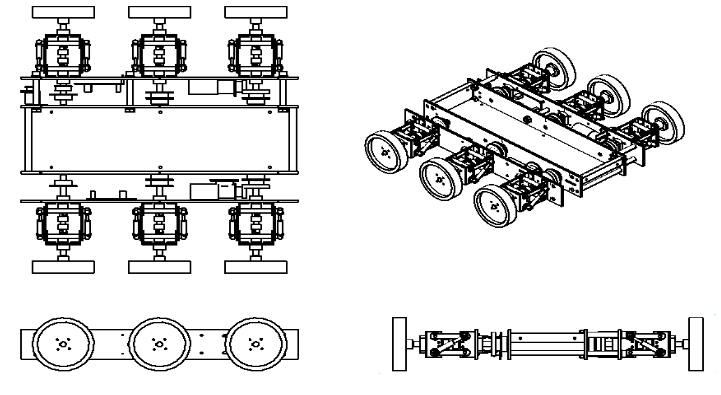
\includegraphics[width=100mm]{img/hard/fig3.png} 
  \caption{6輪ローバ} 
  \label{fig:rokurin}%ここに文章中で使用する名前を指定する 
 \end{center} 
\end{figure} 

\subsection{サスペンションの配置} 
%ダブルウィッシュボーン式サスペンションは便利ではあるが問題点も目立つ.例えばばねのストロークが少ない,ストロークを大きくしようとすれば車体との接続が困難になる,決められた場所にしか設置できない等,どれもスペースが大きく関係してくる. 

ハードウェアの全高は小さくなるため,サスペンションの配置は小スペースに収めることが必要になる.そこで図\ref{fig:box}のように軸棒,ユニバーサルジョイント,車輪を上下のリンクと板を用いて1つの平行リンクをつくり,その平行リンクの両斜辺に2つ直接斜めに振動吸収となるばねを設置すれば車輪の径に左右されるものの従来のものよりスペースが小さく上下機構が得られるのではないかと考えた. 

\begin{figure}[htbt] 
 \begin{center} 
  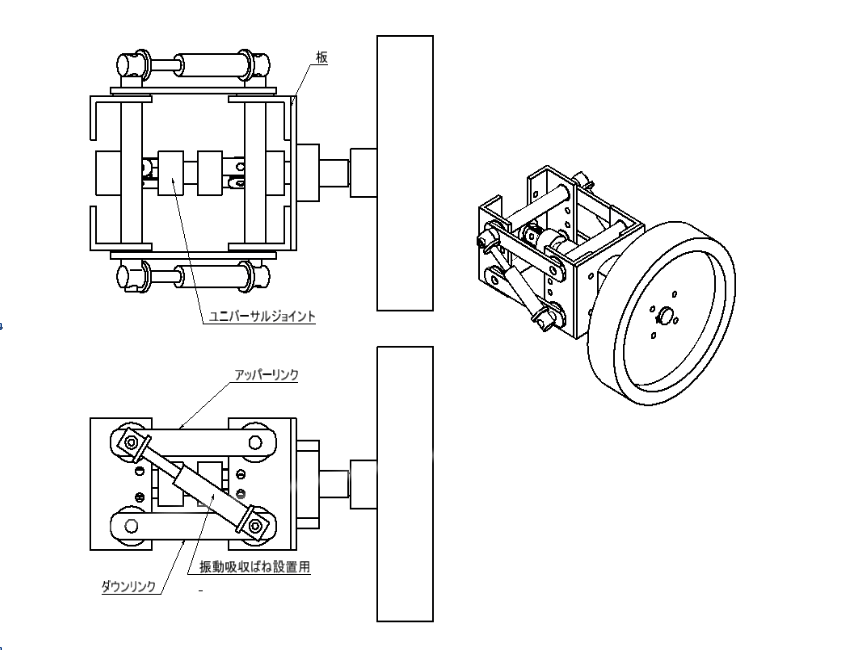
\includegraphics[width=100mm]{img/hard/fig4.png} 
  \caption{平行リンク} 
  \label{fig:box}%ここに文章中で使用する名前を指定する 
 \end{center} 
\end{figure} 

\subsection{ばねのストロークの算出} 
図\ref{fig:bix}に平行リンクの簡易図を示す.また平行リンクが移動した際の図を図\ref{fig:rink}示す.これらの数値よりサスペンションのストロークの長さを求める.サスペンションの全体長さは斜辺に設置するため余弦定理より 
\begin{eqnarray} 
   AC = b^2 & = & a_1^2+c^2-2a_1\cdot c\cdot cos\angle B \\ 
  b & = & \sqrt{38^2+60^2-2\cdot 38\cdot 60\cdot cos90} \\ 
    & = &71.022 ≒ 71.0[mm] 
\end{eqnarray} 
となる.また今回は30[mm]程度の障害物を乗り越える想定しているため,この平行リンクが点A,Bを回転軸として点C,Dが30[mm]上昇した際の平行四辺形の斜辺AC'を求める必要がある.平行リンクが移動してできるΔAC'Eの斜辺AC'はΔAD'Eの辺d'に等しい.よってAC'の式は余弦定理と代入法より 
\begin{eqnarray} 
	AE& = &d' =  \sqrt{a_2^2+e_1^2-2a_2\cdot e\cdot cos\angle D} \\ 
	d' & = & c' \\ 
	AC'&= &e_2  =  \sqrt{c'^2+a_3^2-2\cdot c'\cdot a_3\cdot cos\angle E} 
\end{eqnarray} 
となる.またΔAD'Eの\[\angle A\]は30[mm]上がった際に30[deg]になることから,斜辺AC'は 
\begin{eqnarray} 
	d' &=& \sqrt{30^2+60^2-2\cdot 30\cdot 60\cdot cos\angle 60} \\ 
	d'&=&30\sqrt{3}=c' \\ 
	AC'&= &e_2  =  \sqrt{c'^2+a_3^2-2\cdot c'\cdot a_3\cdot cos\angle E}  \\ 
	AC' &=& \sqrt{(30\sqrt{3})^2+8^2-2\cdot 30\sqrt{3}\cdot 8\cdot cos90} \\ 
	& = & 52.574 ≒ 52.6 [mm] 
\end{eqnarray} 
となる. \\ 
サスペンションは伸縮するものであり,それはこれらの辺ACと辺AC'の差分だけ変化することになる.今回の値から変化値x≒18[mm]程度の変化があることが確認された.以上のAC,AC',xを用いてサスペンションの細かい設計を行う. 

\begin{figure}[htp] 
 \begin{center} 
  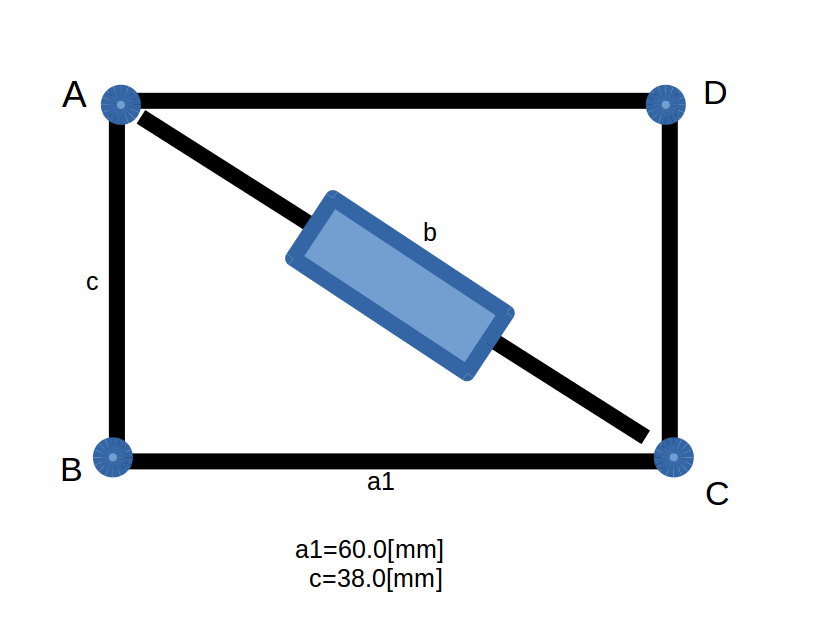
\includegraphics[width=100mm]{img/hard/fig5.png} 
  \caption{平行リンク簡易図} 
  \label{fig:bix}%ここに文章中で使用する名前を指定する 
 \end{center} 
\end{figure} 


\begin{figure}[htp] 
 \begin{center} 
  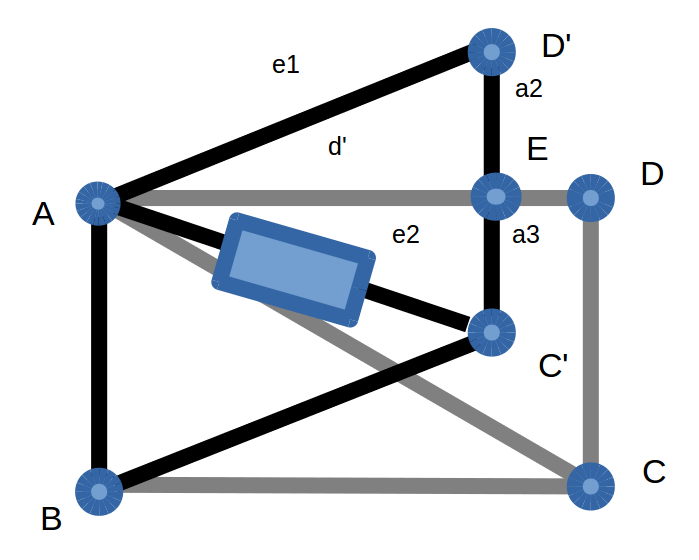
\includegraphics[width=100mm]{img/hard/fig6.png} 
  \caption{平行リンクの移動量変化} 
  \label{fig:rink}%ここに文章中で使用する名前を指定する 
 \end{center} 
\end{figure} 

\subsection{ばね定数の算出} 
サスペンションには路面の凹凸を車体に伝えない緩衝装置としての機能としてばねが必要であるため,フックの法則よりばねを選定する. \\ 
平行リンクの点A,Bをそれぞれ固定支点と考えて計算を行う.図\ref{fig:fbd}に Free Body Diagram(FBD)を示す.図\ref{fig:fbd}よりスラスト方向荷重x,ラジアル方向荷重y,モーメントMの式はそれぞれ 

\begin{eqnarray} 
	x & = & R_AX+R_BX=0 \\ 
	y & = & R_AY+R_BY+F=0 \\ 
	M & = & BC\cdot F-AB\cdot R_AX=0 
\end{eqnarray} 
となる.更に点A,B,Cそれぞれの力は以下のようになる. 

\subsubsection{点Aでの力学計算} 
点Aでは図\ref{fig:bai}より以下のように計算できる. 
\begin{eqnarray} 
	R_AX+FAC\cdot cosθ & = & 0 \\ 
	R_AY & = & FAC\cdot sinθ 
\end{eqnarray} 
\subsubsection{点Bでの力学計算} 
点Bは図\ref{fig:bai}より以下のように計算できる. 
\begin{eqnarray} 
	R_BX+FBC & = & 0 \\ 
	R_BY & = & 0 
\end{eqnarray} 
\subsubsection{点Cでの力学計算} 
点Cは図\ref{fig:bai}より以下のように計算できる. 
\begin{eqnarray} 
	FAC\cdot cosθ+FBC & = & 0 \\ 
	F+FAC\cdot sinθ & = & 0 
\end{eqnarray} 
%\subsubsection{力学計算まとめ} 
上記で求めた式より,ACにかかる力FACの式を計算する. 
FACは式(14)と式(18)より 
\begin{eqnarray} 
	R_AY+F & = & 0 \\ 
		F & = & -R_AY 
\end{eqnarray} 
\begin{eqnarray} 
	    R_AY & = & FAC\cdot sinθ \\ 
		FAC & = & \frac{F}{sinθ} [N] 
\end{eqnarray} 
\begin{eqnarray} 
	F+FAD\cdot sinθ & = & 0 \\ 
	FAC & = & \frac{F}{sinθ} [N] 
\end{eqnarray} 

となることが確認できる. \\ 
力FAC[N]はばね全体に掛る力なので,これをばね1個辺りに加わる力に除算する必要がある.今回作成する6輪ローバは1輪に2つのばねを持つため,ばねを合計で12個保有する.よってばね1個にかかる力FAC[N]は 

\begin{eqnarray} 
	FAC & = & \frac{F}{sinθ}\cdot \frac{1}{12} [N] 
\end{eqnarray} 

となる.今回は重量が15kgになると想定して,ばね定数を求めると 
\begin{eqnarray} 
	FAC & = & \frac{F}{sinθ}\cdot \frac{1}{12} \\ 
	FAC & = & \frac{15 \cdot  9.81}{sin30}\cdot \frac{1}{12} [N] \\ 
	     & =& 24.525[N] 
\end{eqnarray} 
	{これより}  
\begin{eqnarray} 
	k& = &  \frac{F}{x} \\ 
	k& = &  \frac{24.525}{18} \\ 
	 & = & 1.3625 [N/mm] 
\end{eqnarray} 
となる.よってばね定数は1.0[N/mm]の物を採用する. 
\subsection{使用したばね定数} 
上記でばね定数を求めたが,実際に使用した際に車体が沈むのが確認された.想定していた15kgを超えたせいだと考えられる.車体を沈ませないこと,また段差を超えるため車体を浮かせるために2,3N/mmの物を用意し,使用した.結果的に2N/mmは沈まなかったがばねが反発しなかったため,3N/mmのばねを使用することとなった. 

\begin{figure}[htp] 
 \begin{center} 
  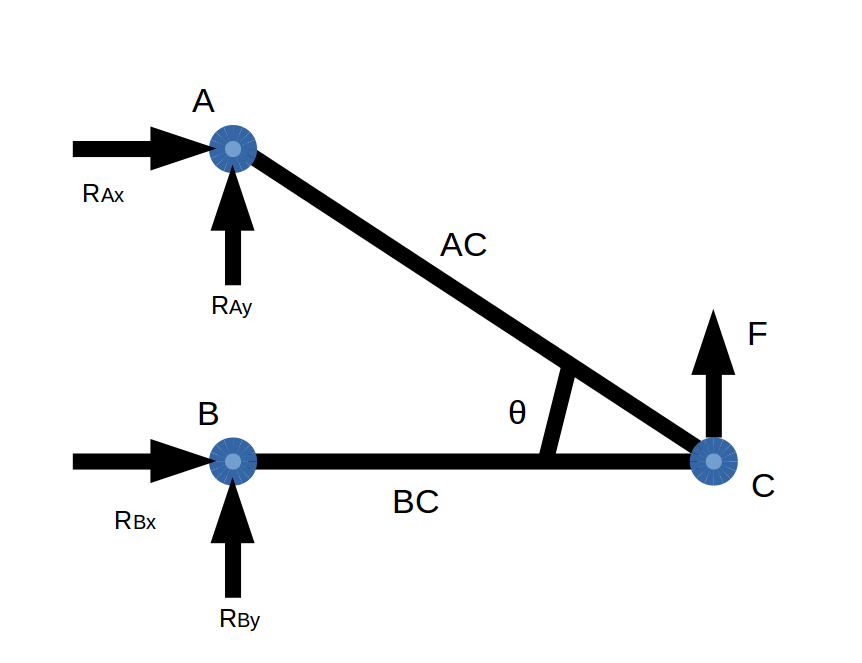
\includegraphics[width=100mm]{img/hard/fig7.png} 
  \caption{FBD} 
  \label{fig:fbd}%ここに文章中で使用する名前を指定する 
 \end{center} 
\end{figure} 

\begin{figure}[htp] 
 \begin{center} 
  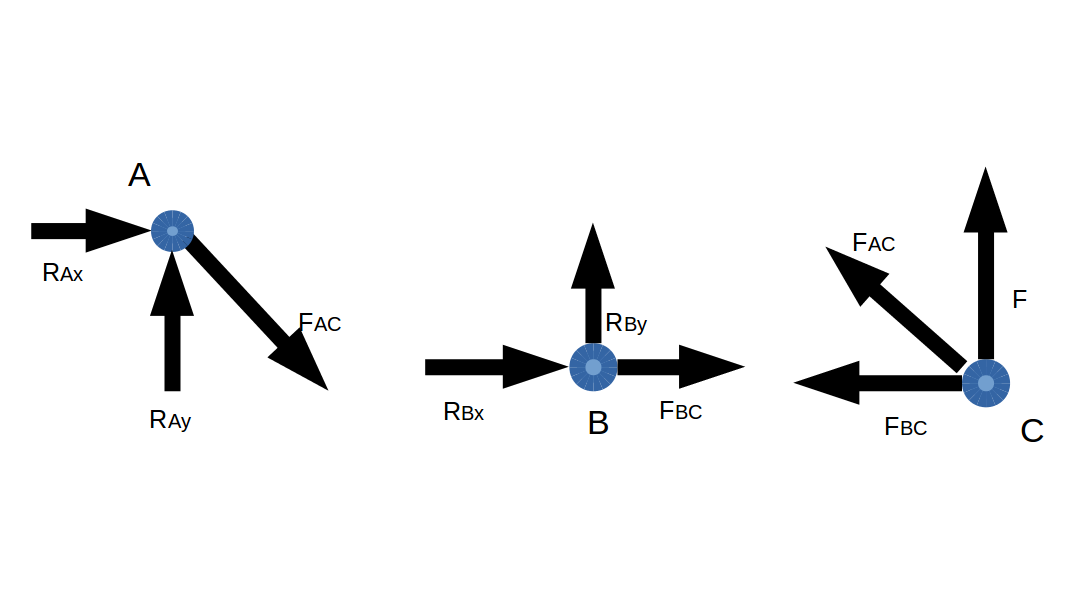
\includegraphics[width=100mm]{img/hard/fig8.png} 
  \caption{各点にかかる力} 
  \label{fig:bai}%ここに文章中で使用する名前を指定する 
 \end{center} 
\end{figure} 




\subsection{低重心化の実現} 
設計した走行モジュールのCADを図\ref{fig:cad}に示す.図から確認できるように全高がタイヤ直径である190mm内に収まっているため低重心化が達成された.また6輪に付属している懸架装置を図\ref{fig:kenka}に示す.ばねを2本設置することでサスペンションとし,またそれらの取り付け位置を斜めにすることでさらに低重心が可能となった. 

\begin{figure}[htp] 
 \begin{center} 
  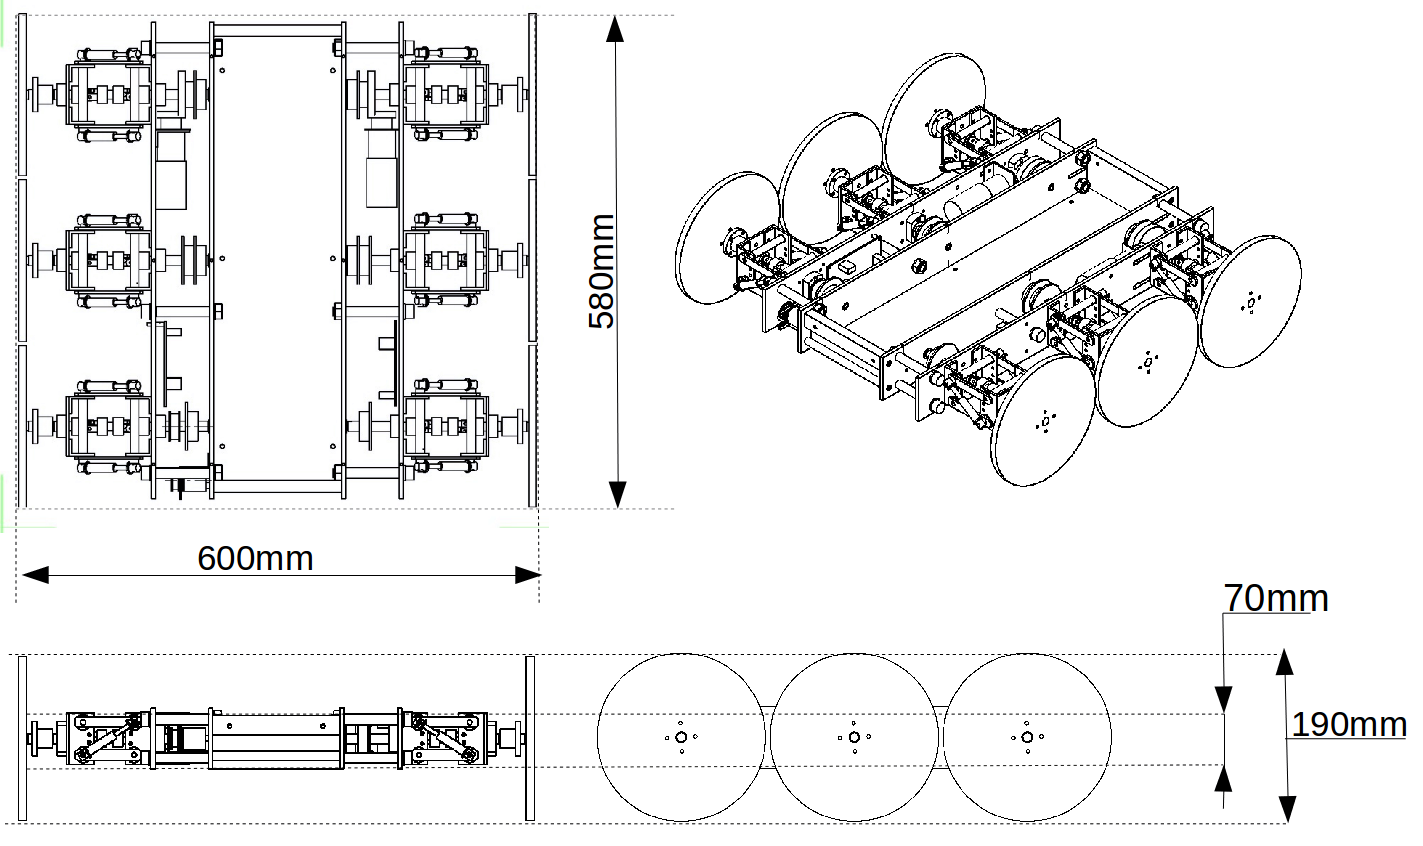
\includegraphics[width=150mm]{img/hard/4.png} 
  \caption{走行モジュール} 
  \label{fig:cad}%ここに文章中で使用する名前を指定する 
 \end{center} 
\end{figure} 

\begin{figure}[htp] 
 \begin{center} 
  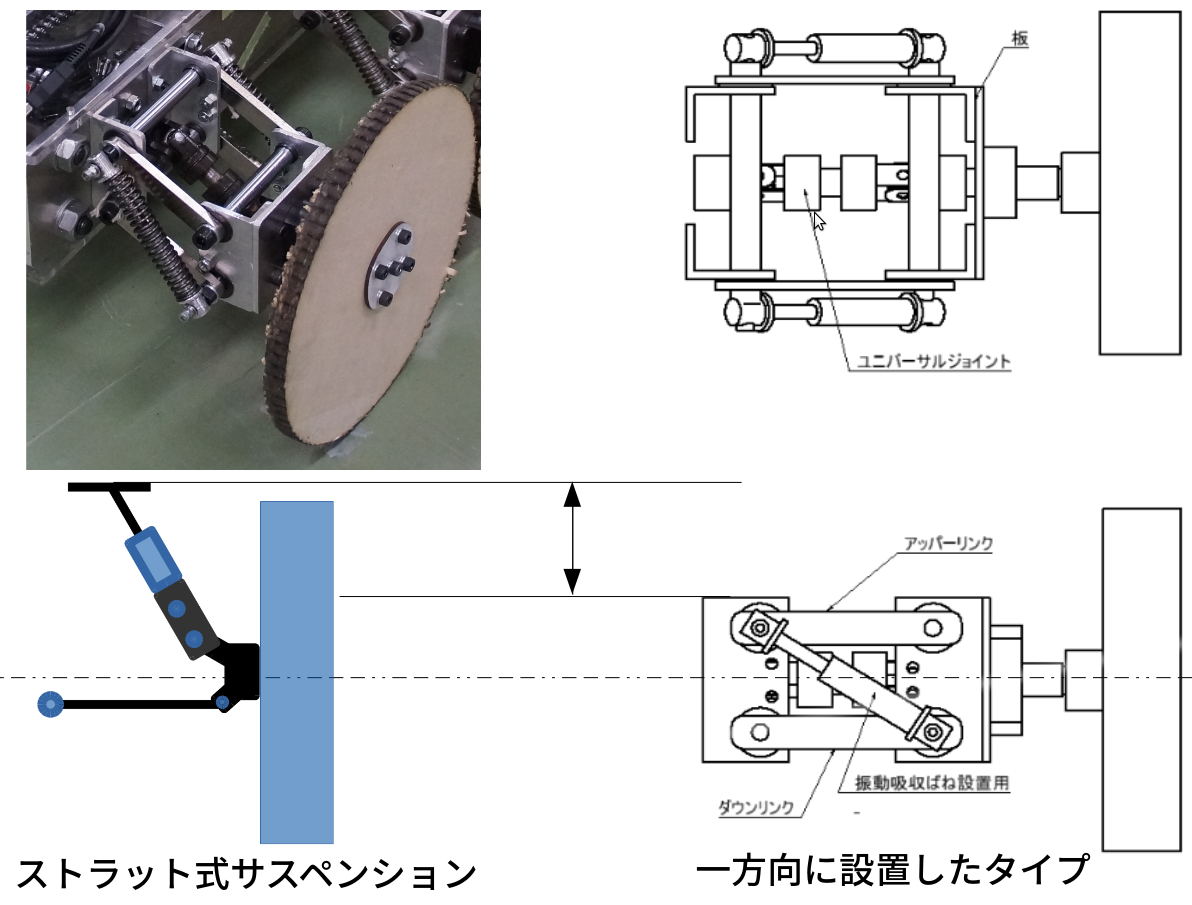
\includegraphics[width=100mm]{img/hard/3.png} 
  \caption{懸架装置} 
  \label{fig:kenka}%ここに文章中で使用する名前を指定する 
 \end{center} 
\end{figure} 


\subsection{超堤・超壕能力} 
今回作成したロボットの性能を調査するため,超堤・超壕実験を行った結果,超堤:110[mm],超壕220[mm]が得られた. 

\subsection{電気設計} 
ロボットに搭載したモータドライバの回路図を図\ref{fig:denkikairo}に示し,使用した部品を表\ref{tab:denkibuhin}に示す.モータドライバは各Dモジュールに1つづつの設置とした. 

\begin{figure}[htp] 
 \begin{center} 
  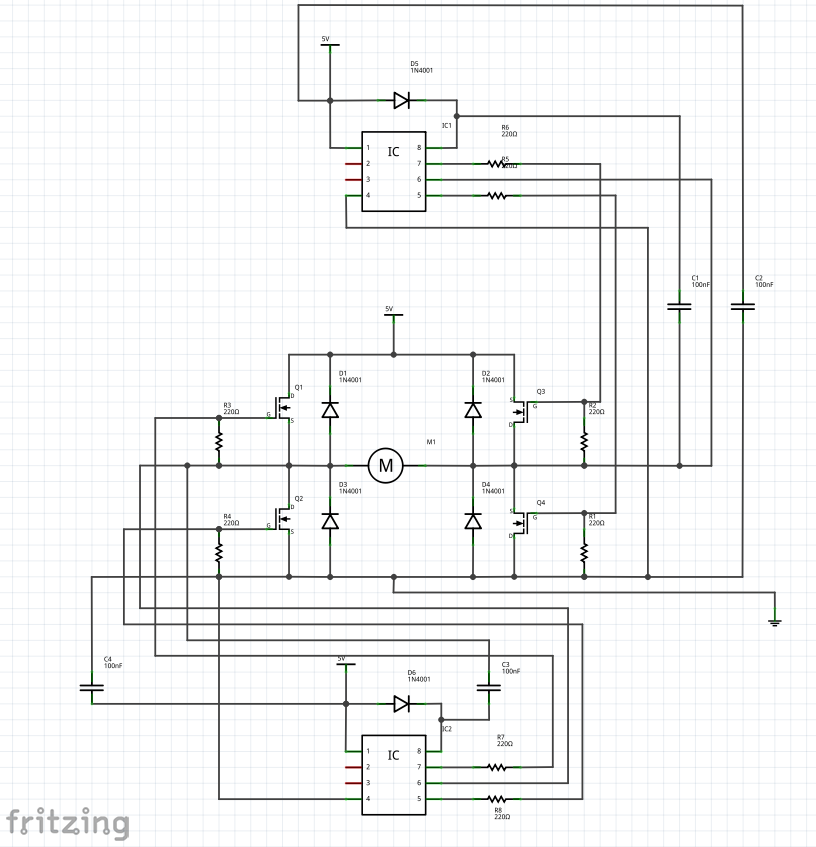
\includegraphics[width=140mm]{img/hard/kairozu.png} 
  \caption{モータドライバ} 
  \label{fig:denkikairo}%ここに文章中で使用する名前を指定する 
 \end{center} 
\end{figure} 


\begin{table}[htp] 
  \begin{center} 
    \caption{使用した電気部品} 
  \begin{tabular}{|c|c|c|} \hline 
品名 & 型番 & メーカ &  \\  \hline 
自作MD板  & \\ \hline 
トロイダルコイル 330μH9A  &  &秋月電子\\ \hline 
EIコネクタ4ピンオス  &  & \\ \hline 
EIコネクタ2ピンオス  & 171825-2 & 秋月電子 \\ \hline 
FET(電界効果トランジスタ) & \\ \hline 
カーボン抵抗 1/4W 47kΩ (100本入) & R-25473 & 秋月電子\\ \hline 
カーボン抵抗 1/4W 47Ω (100本入) &  R-25470 & 秋月電子\\ \hline 
カーボン抵抗 1/4W 10kΩ (100本入) & R-25103 & 秋月電子\\ \hline 
セラミックコンデンサ103 & RPEF11H104Z2P1A01B & 秋月電子 \\ \hline 
セラミックコンデンサ105 & RDEC71E106K2K1C03B & 秋月電子 \\ \hline 
発光ダイオード &  \\ \hline 
RX220マイコンボード & K-08769 & 秋月電子\\ \hline 
  \end{tabular} 
    \label{tab:denkibuhin} 
  \end{center} 
\end{table} 

\section{ソフト}
\subsection{使用ソフトウェア} 
ロボットのソフトウェアにはUbuntu 14.04とGNU Compilerを用いる.また使用言語はC++言語である. 

\subsection{使用したライブラリ} 
表\ref{tab:op}に使用したライブラリを示す. OpenCVは画像処理・画像解析および機械学習等の機能を持つC/C++,Java,Python,MATLAB用ライブラリであり,後述するマップ作成の主に画像処理に用いる. Point Cloud Librayとは2,3次元の点群からフィルタリング,特徴推定,サーフェス再構成,レジストレーション(位置合わせ),モデルフィッティング,セグメンテーションなどのアルゴリズムが使用できる.これはOpenCVから得られた点情報を画面上に表示するために使用する. Urg libraryとはレーザ距離センサ URG シリーズ用のオープンソースライブラリである.今回は障害物回避のため用いる. 
\begin{table}[h] 
  \begin{center} 
    \caption{使用したライブラリ} 
    \small 
  \scalebox{1.00}{ 
  \begin{tabular}{|c|c|} \hline 
    ライブラリ &  使用用途 \\ \hline 
    OpenCV 3.00 &  画像処理\\ \hline 
    Point Cloud Library 1.7 &  点群管理 \\ \hline 
    urg library 1.2.0 &  障害物回避 \\ \hline 

  \end{tabular} 
  } 
    \label{tab:op} 
  \end{center} 
\end{table}

\chapter{単眼カメラによる三次元測量}
\section{カメラの幾何学}
カメラの姿勢を並進・回転の同次変換行列で表したものを外部パラメータ行列Eという.
また,カメラの焦点距離と画像中心座標をピクセル単位で4×4行列の形に表したものを内部パラメータ行列Kと呼ぶ.
さらに,三角測量を行う際に用いる情報をまとめた行列を射影変換行列Hと呼びこれらの関係を以下に示す.ただし,この時の焦点距離と中心座標は(fx,fy),(cx,cy)とする.

\begin{eqnarray}
  K = \left(
    \begin{array}{cccc}
      fx & 0 & cx & 0\\
      0 & fy & cy & 0\\
      0 & 0 & 1 & 0\\
      0 & 0 & 0 & 1
    \end{array}
  \right)
\end{eqnarray}
\begin{eqnarray}
  E = \left(
    \begin{array}{cccc}
      r_{11} & r_{12} & r_{13} & t_1\\
      r_{21} & r_{22} & r_{23} & t_2\\
      r_{31} & r_{32} & r_{33} & t_3\\
      0 & 0 & 0 & 1
    \end{array}
  \right)
\end{eqnarray}
\begin{eqnarray}
  H = KE
\label{eqnarray:H}
\end{eqnarray}

これらの関係から射影変換行列Hを求める.
\section{三角測量の原理}
三角測量とは座標が既知の2点とそれらの点間距離,それぞれの点と対象物との角度から正弦定理を用いて対象物の座標を得るものである.
カメラでは対象物を写した2枚の画像と射影変換行列から三角測量を行うことができる.以下にその原理を図\ref{fig:sankaku1}として示す.
図より三角測量の原理を用いて対象物の座標は以下の式で求めることができる.
\begin{eqnarray}
	X&=&\frac{L(X_l+X_r)}{2(X_l-X_r)}\\
	Y&=&\frac{L(Y_l+Y_r)}{2(X_l-X_r)}\\
	Z&=&\frac{fL}{X_l-X_r}
\end{eqnarray}
よって射影変換行列とカメラ間の距離を求めることで対象物の座標がわかる.

\begin{figure}[htp]
 \begin{center}
  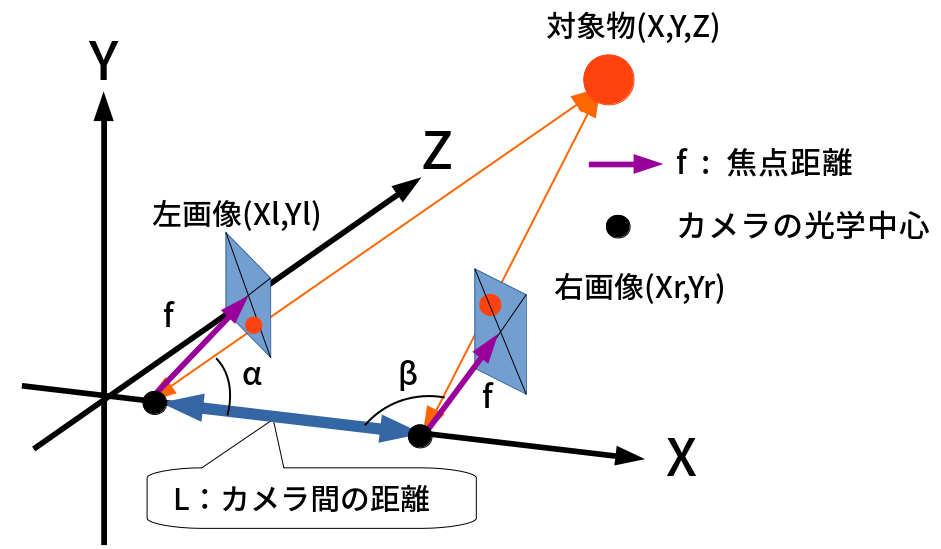
\includegraphics[width=120mm]{img/soft/sankaku2.png}
  \caption{三角測量の原理}
  \label{fig:sankaku2}%ここに文章中で使用する名前を指定する
 \end{center}
\end{figure}

\section{単眼カメラによる三角測量}
図\ref{fig:sankaku1}のように三角測量を行う際には2つのカメラを用いるのが一般的だ.だが今回はカメラを移動させ過去の位置で取得した画像を利用することで単眼カメラで三角測量を行えるようにした.この原理を図\ref{fig:sankaku2}に示す.図\ref{fig:sankaku2}より,カメラ間の距離はカメラの移動量に等しい.また,カメラが定点でなく移動するため外部パラメータ行列が変化する.
このことから単眼カメラで三角測量を行うためには射影変換行列とカメラの移動量をリアルタイムで得る必要がある.

\begin{figure}[htp]
 \begin{center}
  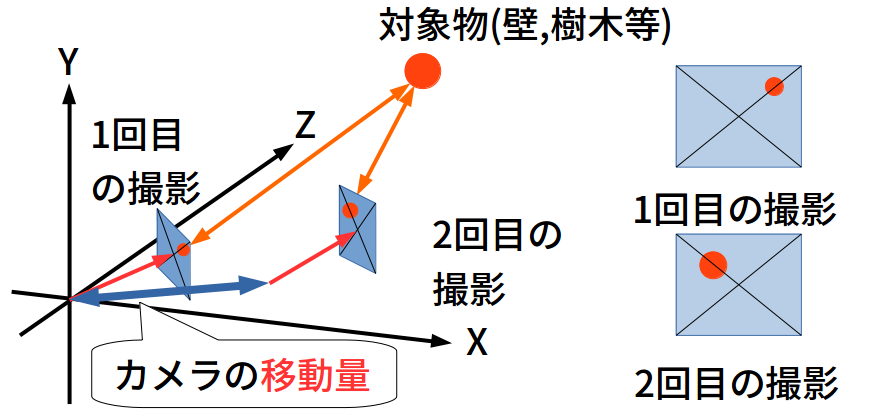
\includegraphics[width=120mm]{img/soft/sankaku1.png}
  \caption{単眼カメラによる三角測量}
  \label{fig:sankaku1}%ここに文章中で使用する名前を指定する
 \end{center}
\end{figure}

\section{射影変換行列の算出}
\subsection{内部パラメータ行列の算出}
OpenCVで内部パラメータ行列を求めることができる関数が用意されている.この関数は8点法\cite{fivepoint}を用いており,同じカメラで撮影した2枚の画像の対応付けられた点の座標を与えることによって内部パラメータ行列を算出することができる.
今回はチェッカーボード画像を用いて,2画像上のチェッカーボードのコーナー座標を検出しそれらを対応付けられた点座標とした.
\subsection{外部パラメータ行列の算出}
OpenCVでは外部パラメータ行列を求めることができる関数が用意されている.この関数は5点法\cite{fivepoint}を用いており,内部パラメータ行列,2枚の画像の対応付けられた点の座標を与えることによって外部パラメータ行列を算出することができる.

\subsection{特徴点抽出}

座標が既知の2点を算出するためにそれぞれ2枚の画像から特徴的な点を抽出する必要がある.本論文ではOpenCVで使用可能な既存のアルゴリズムを用いて特徴点を抽出する.OpenCVで使用可能なアルゴリズムには様々な種類がありそれぞれ異なった特徴を持っている.以下に代表的なアルゴリズムとその特徴をまとめ表\ref{tab:SURF}として示す.これらのアルゴリズムは基本的に画像内の明暗から角(エッジ)を検出している.そのため色情報を用いないことが多く,計算量削減のためモノクロ画像が用いられることが多い.

\begin{table}[h] 
  \begin{center} 
    \caption{代表的な特徴点抽出アルゴリズム} 
    \small 
  \scalebox{1.00}{ 
  \begin{tabular}{|c|c|} \hline 
    アルゴリズム &  備考 \\ \hline 
    SIFT,SURF & 照明変化に頑健で回転,拡大縮小に不変であるが計算量が多い.SURFはSIFTの改良版 \\ \hline 
    ORB &  局所性鋭敏型ハッシュという手法を用いており,計算量が少ない \\ \hline 
    FAST &  回転に不変である. \\ \hline
    KAZE,AKAZE & SIFTに比べ,ロバスト性の向上と計算量削減を重視 AKAZEはKAZEの改良版\\ \hline
 

  \end{tabular} 
  } 
    \label{tab:SURF} 
  \end{center} 
\end{table}

今回は外で使用するため照明変化に頑健なアルゴリズムのうち計算量を削減したSURFを使用する.


\subsection{特徴点の対応付け}

\begin{figure}[htp]
 \begin{center}
  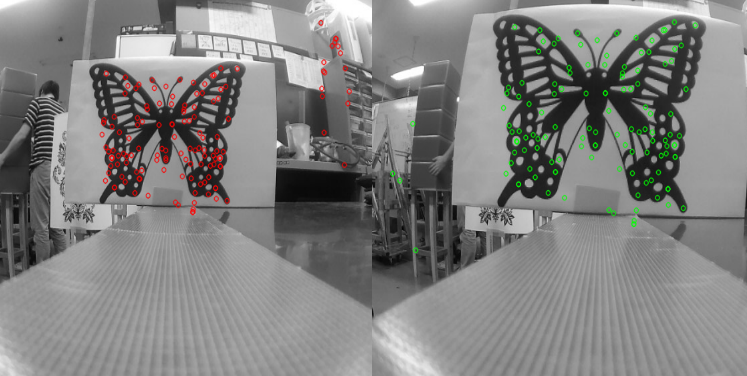
\includegraphics[width=120mm]{img/soft/surf.png}
  \caption{特徴点の抽出}
  \label{fig:surf}%ここに文章中で使用する名前を指定する
 \end{center}
\end{figure}

1枚目の画像から抽出した特徴点が2枚目の画像のどこに対応しているのかを知るためにk近傍法(k nearest neighbor)を使用する.
1枚目の画像のある特徴点を

\begin{eqnarray}
	\vec{a}  & = & (a_1, a_2 \cdots, a_n)
\end{eqnarray}

2枚目の画像のある特徴点を

\begin{eqnarray}
	\vec{b}  & = & (b_1, b_2 \cdots, b_n)
\end{eqnarray}

とすると
以下のように各特徴点の成分を差分し三平方の定理を用いることで対応している点の候補をk個(kは任意)算出する.

%k近傍法によって抽出したすべての特徴点から特徴量と呼ばれる特徴点を構成するベクトルの差分が最も小さい上位k個(kは指定可能)を

\begin{eqnarray}
	d & = & \sqrt{(a_1-b_1)^2+ (a_2-b_2)^2 \cdots+ (a_n-b_n)^2}
\end{eqnarray}

この手法を用いて2枚の蝶が写っている画像を対応付けし,描画した画像を図\ref{fig:chou}に示す.

\begin{figure}[htp]
 \begin{center}
  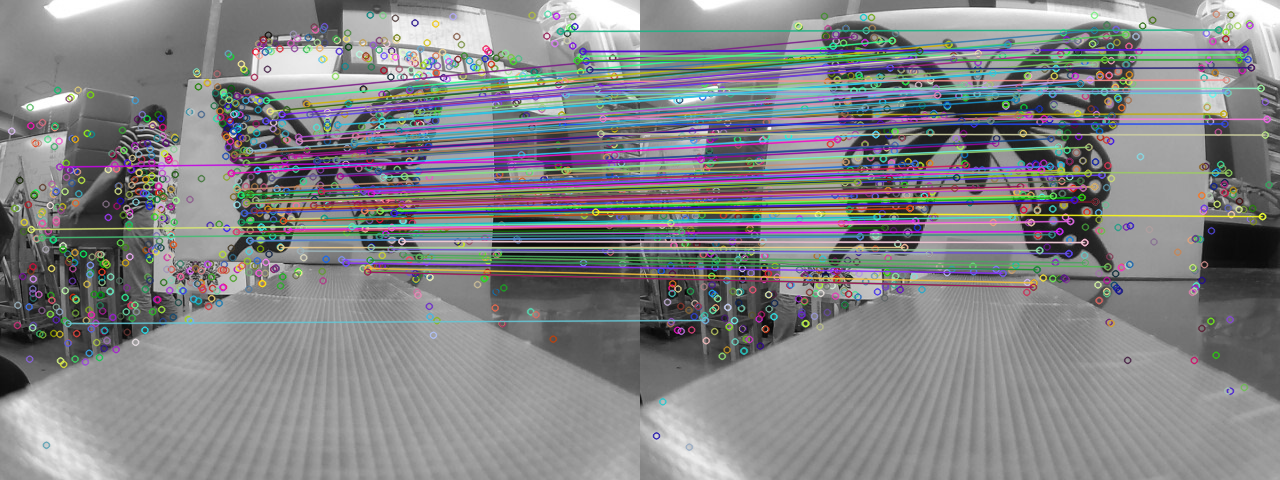
\includegraphics[width=120mm]{img/soft/chou.png}
  \caption{特徴点の対応付け}
  \label{fig:chou}%ここに文章中で使用する名前を指定する
 \end{center}
\end{figure}

図\ref{fig:chou}のように,座標が既知の2点を多数算出することができた.

\subsection{射影変換行列の算出}

前述のように2枚の画像の対応付けられた点座標と内部パラメータ行列を得ることができた.これより前述のOpenCVの関数を用いることで外部パラメータ行列を算出することができる.
よって,式\ref{eqnarray:H}を用いて射影変換行列を求めることができる

\section{移動量の取得}
カメラの移動量を取得するため,東京航空計器社製のモーションセンサから得られる位置情報を使用する.モーションセンサーを図\ref{fig:motion}に示す.1回目に取得した位置と2回目に取得した位置の
差から移動量を算出する.

\begin{figure}[htp]
 \begin{center}
  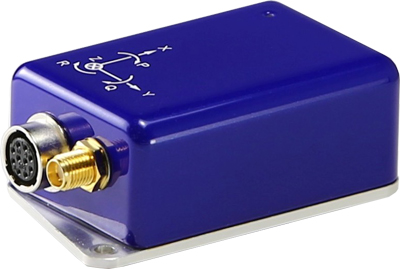
\includegraphics[width=50mm]{img/soft/motion.jpg}
  \caption{モーションセンサー}
  \label{fig:motion}%ここに文章中で使用する名前を指定する
 \end{center}
\end{figure}

\subsection{地平直行座標への変換}
モーションセンサーから得られる緯度,経度,高度をメートル単位に変換することによって,1回目に取得した位置と2回目に取得した位置からどれくらい移動したのかが分かりやすくなる.そのためには緯度,経度,高度から地平直交座標系に変換する必要がある.地平直行座標への変換の模式図を図\ref{fig:zahyou}に示す.


\begin{figure}[htp]
 \begin{center}
  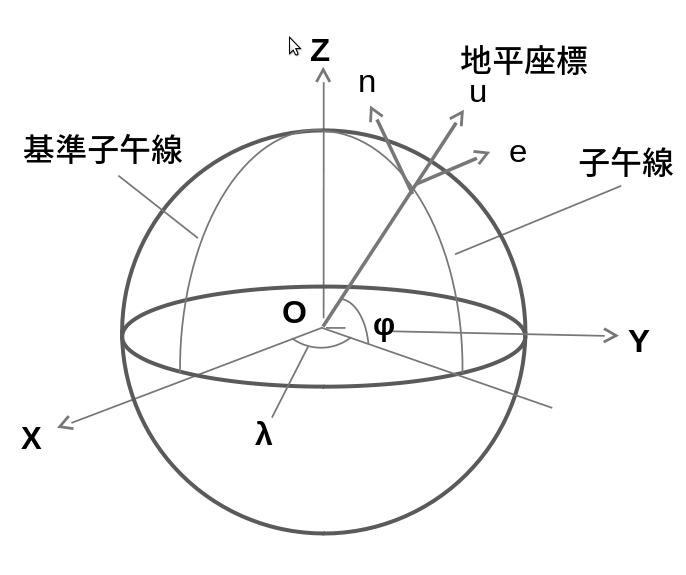
\includegraphics[width=80mm]{img/soft/zahyou.png}
  \caption{地平座標への変換}
  \label{fig:zahyou}%ここに文章中で使用する名前を指定する
 \end{center}
\end{figure}

地平直行座標に変換する際には地球重心を原点とした x y z 座標であるECEF(earth centered, earth fixed)座標に変換する必要がある.
緯度をφ,経度をλ,高度をhとし x y z を求めるために係数Nを求める.
離心率をe,偏平率をfとすると係数Nは式\ref{fig:keisu}によって求めることができる.
\begin{eqnarray}
	N  & = & \frac{a}{\sqrt{1-e^2\sin^2\phi}}
	\label{fig:keisu}
\end{eqnarray}
この係数Nを使用し, x y zそれぞれの座標を求めることができる.
\begin{eqnarray}
	x  & = & (N+h)\cos\phi\cos\lambda
\end{eqnarray}
\begin{eqnarray}
	y  & = & (N+h)\cos\phi\sin\lambda
\end{eqnarray}
\begin{eqnarray}
	z  & = & \{N(1-e^2)+h\}\sin\phi
\end{eqnarray}
上記の式より求めた x y z 座標から地平直行座標に変換する.ECEF直交座標から地平直交座標への変換は,回転と原点移動のみによって実現される.地平座標での位置(e, n, u)は,ECEF直交座標での位置(x, y, z)と原点の位置(x{\scriptsize 0}, y{\scriptsize 0}, z{\scriptsize 0})で,式で求めることができる.
\begin{eqnarray}
  \left(
    \begin{array}{c}
      e\\
      n\\
      u\\ 
    \end{array}
  \right)=R(z,90)R(y,90-\phi)R(z,\lambda)
  \begin{pmatrix}
      x-x_0\\
      y-y_0\\
      z-z_0 
    \end{pmatrix}
\end{eqnarray}

これによって得られた位置(e, n, u)から三平方の定理を用いて距離を算出する.



\chapter{マップ生成}

\section{マップ生成環境}
マップの生成環境を図\ref{fig:map}に示す.天候はカメラ画像に影響の少ないくもりの日,画像間距離を1.4[m]として金沢工業高等専門学校の駐車場付近でマップ生成を行った.ロボットはStart地点から矢印の方向に進み,2回の旋回を経てGoal地点まで走行する.

\begin{figure}[htp]
 \begin{center}
  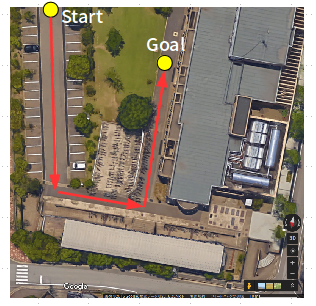
\includegraphics[width=80mm]{img/soft/1.png}
  \caption{マップ生成環境}
  \label{fig:map}%ここに文章中で使用する名前を指定する
 \end{center}
\end{figure}

\section{マップ生成}
生成されたマップを図\ref{fig:mapp}に示す.赤い点群はカメラ画像から三角測量によって得られた周囲の位置関係,青い線はカメラ画像から得られたロボットの走行軌跡,黄色い線を実際にロボットが走行した軌跡である.
図より,カメラ画像からマップを生成することができた.
しかしカメラ画像から得られたロボットの走行軌跡は1回目の旋回時から,実際にロボットが走行した軌跡と比べて大きく歪んでいることが確認できる.

\begin{figure}[htp]
 \begin{center}
  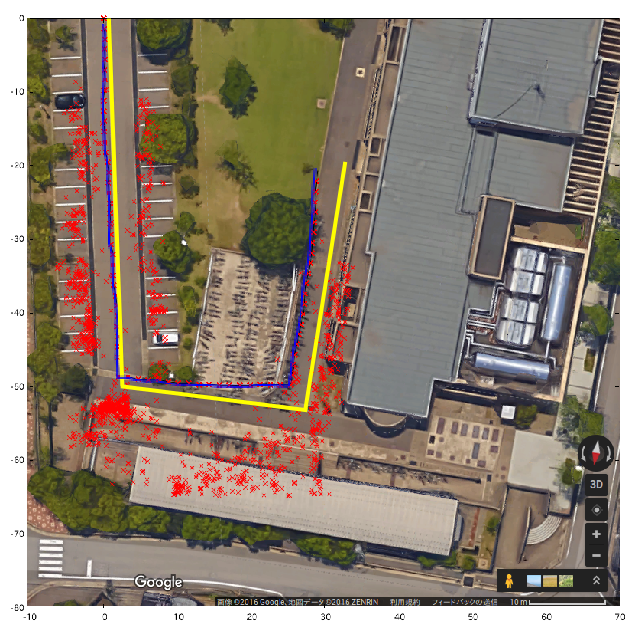
\includegraphics[width=80mm]{img/soft/2.png}
  \caption{生成したマップ}
  \label{fig:mapp}%ここに文章中で使用する名前を指定する
 \end{center}
\end{figure}

\section{移動量のばらつき}
マップ生成を行った際にモーションセンサーから得られた移動量のばらつきを図\ref{fig:gps}に示す.

\begin{figure}[htp]
 \begin{center}
  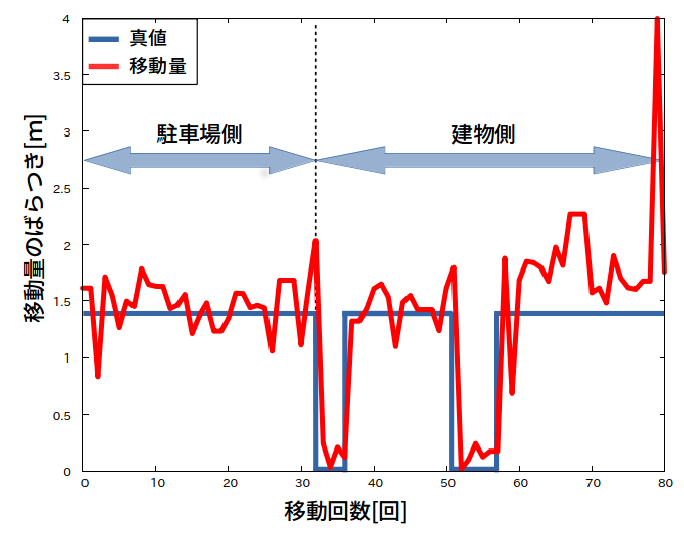
\includegraphics[width=80mm]{img/soft/gps.png}
  \caption{移動量のばらつき}
  \label{fig:gps}%ここに文章中で使用する名前を指定する
 \end{center}
\end{figure}

図を見て分かるとおり,駐車場側では取得した移動量が真値から増減しているためマップ生成をした際のズレが小さい.しかし建物側に近づくに連れて取得した移動量が真値よりも大きく増加してしまっている.また旋回時は移動を行っていないため移動量は0[m]になっている必要があるのに対し,取得した移動量は0[m]になっておらず,これらの原因によってマップ生成の際にズレが発生してしまったと考えられる.

\chapter{結言}
\section{本研究のまとめ}
走破性の高いロボットの開発の実現にあたり,つくば市内での走行が問題なく行えたため,走破性の高いロボットの開発は達成したと考える.また移動量の取得とマップ生成の実現にあたり,生成したマップは旋回時に大きく歪むことが確認されたが直線時には問題がなかったため3次元復元技術の基礎は確立できたと考える.

\section{今後の課題}
\subsection{自己位置推定}
現在作成できたマップには旋回時に大きく歪むという欠点がある.そのため旋回時には他のセンサーからの情報で外部パラメータ行列に補正をかける必要がある.そこで,今回はタイヤの滑りが原因で使用できなかったがエンコーダなどを使用する方法が考えられる.また,マップ作成時に使用した画像から一定間隔でテンプレート画像を抽出しそれと現在の画像をテンプレートマッチングできれば,対応したテンプレート画像の位置から自己位置を推定できる.この場合,現在の画像とテンプレート画像は鳥瞰図のように同じ視点からの画像になるように透視変換する必要があるが,前後のテンプレート画像に比較対象を絞ることができるため精度が高くなると考えられる.ただし,スタート時には参照できる前後のテンプレート画像を自力で用意できない問題がある他,テンプレートマッチング自体の計算量が多く,処理時間がかかってしまうことが考えられる.

\subsection{タイヤ素材検討}
ロボットのタイヤは木材で作成している.その理由は,ロボットに合うタイヤが見つからず,金沢工業高等専門学校に新しく導入されたレーザー加工機の試験的運用を兼ねて木材で作成した.しかし木材のタイヤでは路上を走行した際に削れる,滑るなどの問題が発生し,タイヤの交換が必要となってしまう.よって削れる,滑ることのないタイヤ素材の検討が必要である.

\subsection{屋内対応}
今回我々は移動量を取得するためにGPSから得られる位置情報を使用しているため,GPSを取得することができない屋内などでは移動量を取得することができない.そこで我々が使用したモーションセンサーは位置情報以外にも加速度や姿勢なども取得することができるため,これらのセンサー情報から屋内でも移動量を取得し屋内マップを生成する.

\subsection{全天候性の付与}
現状では,カメラで周囲の環境を撮影した際に天候によっては周囲の環境を上手く写しだすことができない可能性がある.写り方によってはマップを生成できないため,写り方が天候によって作用されない手段を考える必要がある.

% 参考文献
\begin{thebibliography}{8}
%  \bibitem{harris} LandingProducts, APCPro\nolinebreak pellers,\nolinebreak
%http://www.\linebreak apcprop. com{\slash}v{\slash}index.html,
%2012/8/21
%\bibitem{kyonenn} GPS測位計算プログラム入門,ROS,http://www.enri.go.jp/~fks442/K_MUSEN
\bibitem{ros} Bradski,Kaehler:詳解 OpenCV,433,株式会社オライリー・ジャパン(2012)
\bibitem{kyonenn} 理解するためのGPS測位計算プログラム入門,http://www.enri.go.jp/~fks442/K\_MUSEN
\bibitem{fivepoint} 初期値推定付非線形最小二乗法による5点法の解法
%  \bibitem{koukuu} 中村 資郎:新航空工学講座 第7巻 プロペラ:日本航空技術協会,pp.23-24,1988
%  \bibitem{rikigaku} 加藤 寛一郎,大屋 昭男,柄沢 研治:航空機力学入門,東京大学出版会,pp.32,1982
\end{thebibliography}



\chapter*{謝辞}
\addcontentsline{toc}{chapter}{謝辞}
本論文作成にあたりテーマの決定,研究の考え方,方法のまとめ方など全てにおいて長期にわたって厳しくも熱意のあるご指導,ご鞭撻していただいた,伊藤恒平教授に厚く御礼申し上げます.


特に分析においても論文の書き方においても論文を何度も読んでいただき,指導していただいた伊藤恒平教授に大変ご苦労をかけてしまいましたことにも心よりお詫び申し上げたいです.


同級生のメンバーには論文の作成,修正にご協力いただき心より感謝しております.
その他,助けていただいた多くの皆様に心から感謝しております.ありがとうございました.
%\section{今後の課題}
\subsection{自己位置推定}
現在作成できたマップには旋回時に大きく歪むという欠点がある.そのため旋回時には他のセンサーからの情報で外部パラメータ行列に補正をかける必要がある.そこで,今回はタイヤの滑りが原因で使用できなかったがエンコーダなどを使用する方法が考えられる.また,マップ作成時に使用した画像から一定間隔でテンプレート画像を抽出しそれと現在の画像をテンプレートマッチングできれば,対応したテンプレート画像の位置から自己位置を推定できる.この場合,現在の画像とテンプレート画像は鳥瞰図のように同じ視点からの画像になるように透視変換する必要があるが,前後のテンプレート画像に比較対象を絞ることができるため精度が高くなると考えられる.ただし,スタート時には参照できる前後のテンプレート画像を自力で用意できない問題がある他,テンプレートマッチング自体の計算量が多く,処理時間がかかってしまうことが考えられる.

\chapter*{付録}
\addcontentsline{toc}{chapter}{付録}
\appendix{付録}%%%%%%%%この先付録%%%%%%%%%%%%%%%%%%%%%%%%%%%%%%%%%%%%%%%%%%%%%%
\section{OpenCVのインストール}
今回はUbuntuでOpenCVをインストールする手順を示す.基本的に以下のコマンドをcopy and pasteすればインストールが完了する.
\subsection{必要なファイルをインストールする}
\begin{itemize}
\item 開発ツール

sudo apt-get -yV install cmake libeigen3-dev

ubuntu 16.04以降
sudo apt -yV install cmake libeigen3-dev

\item GUIフレームワーク関連

sudo apt-get -yV install libgtk2.0-dev libgtkglext1-dev libqt4-dev freeglut3-dev


ubuntu 16.04以降
sudo apt -yV install libgtk2.0-dev libgtkglext1-dev libqt4-dev freeglut3-dev

\item 並列処理関連

sudo apt-get -yV install opencl-headers libtbb-dev

ubuntu 16.04以降
sudo apt -yV install opencl-headers libtbb-dev

\item 画像フォーマット関連

sudo apt-get -yV install libjpeg-dev libjasper-dev libpng++-dev libtiff-dev libopenexr-dev libwebp-dev
ubuntu 16.04以降
sudo apt -yV install libjpeg-dev libjasper-dev libpng++-dev libtiff-dev libopenexr-dev libwebp-dev


\item Python関連

sudo apt-get -yV install libpython3.4-dev python-numpy python-scipy python-matplotlib python3-numpy python3-scipy python3-matplotlib

ubuntu 16.04以降
sudo apt -yV install libpython3.4-dev python-numpy python-scipy python-matplotlib python3-numpy python3-scipy python3-matplotlib

\item Qt関連

sudo apt-get -yV install qtbase5-dev
ubuntu 16.04以降

sudo apt -yV install qtbase5-dev

\item cmake-guiインストール

sudo apt-get -yV install cmake-gui
ubuntu 16.04以降

sudo apt -yV install cmake-gui

\end{itemize}
\subsection{GitHubからOpenCVをクローンする}

git clone https://github.com/Itseez/opencv.git

git clone https://github.com/Itseez/opencv\_contrib.git

\subsection{クローンしたOpenCVに移動しビルド用のフォルダを作成する}

cd opencv

mkdir build

\subsection{CMame-guiを実行する}
cmake-gui

\subsection{CMake-guiを以下の手順で操作する}

\begin{enumerate}
\item Where is the source code:にopencvディレクトリまでのパスを指定する

例) /home/kouhei/work/opencv

\item Where to build the binarise:にビルドしたものを置くディレクトリを指定する.先に作ったbuildディレクトリを指定する.

例) /home/kouhei/work/opencv/build

\item configureボタンを押す

\item OPENCV\_EXTRA\_MODULES\_PATHにopencv\_contrib/modulesまでのパスを指定する.

例) /home/kouhei/work/opencv\_contrib/modules

\item Configureボタンを押す

\item Generateボタンを押す

\item cmake-gui終了

\end{enumerate}

\subsection{OpenCVをコンパイル,インストールする}

sudo make install

\subsection{共有ライブラリの依存情報を更新して終了}

sudo ldconfig


\section{ロボットの起動方法}
ロボットが起動するまでに必要な手順を以下に示す.
また,ロボットを起動する際に使用する操作パネルの写真を図\ref{fig:start_panel}に示す.さらに,起動用の外付けSSDを図\ref{fig:start_hdd}に示す.
\subsection{起動}
\begin{enumerate}
\item 操作パネルのうち左上の電源スイッチをonにする.
\item 起動用の外付けSSDが接続されていない場合のみキーボードを接続し「s」と入力する.
\item ロボットから「ubuntuが起動しました」という音声が聞こえるまで待機する.
\end{enumerate}

\begin{figure}[htp]
 \begin{center}
  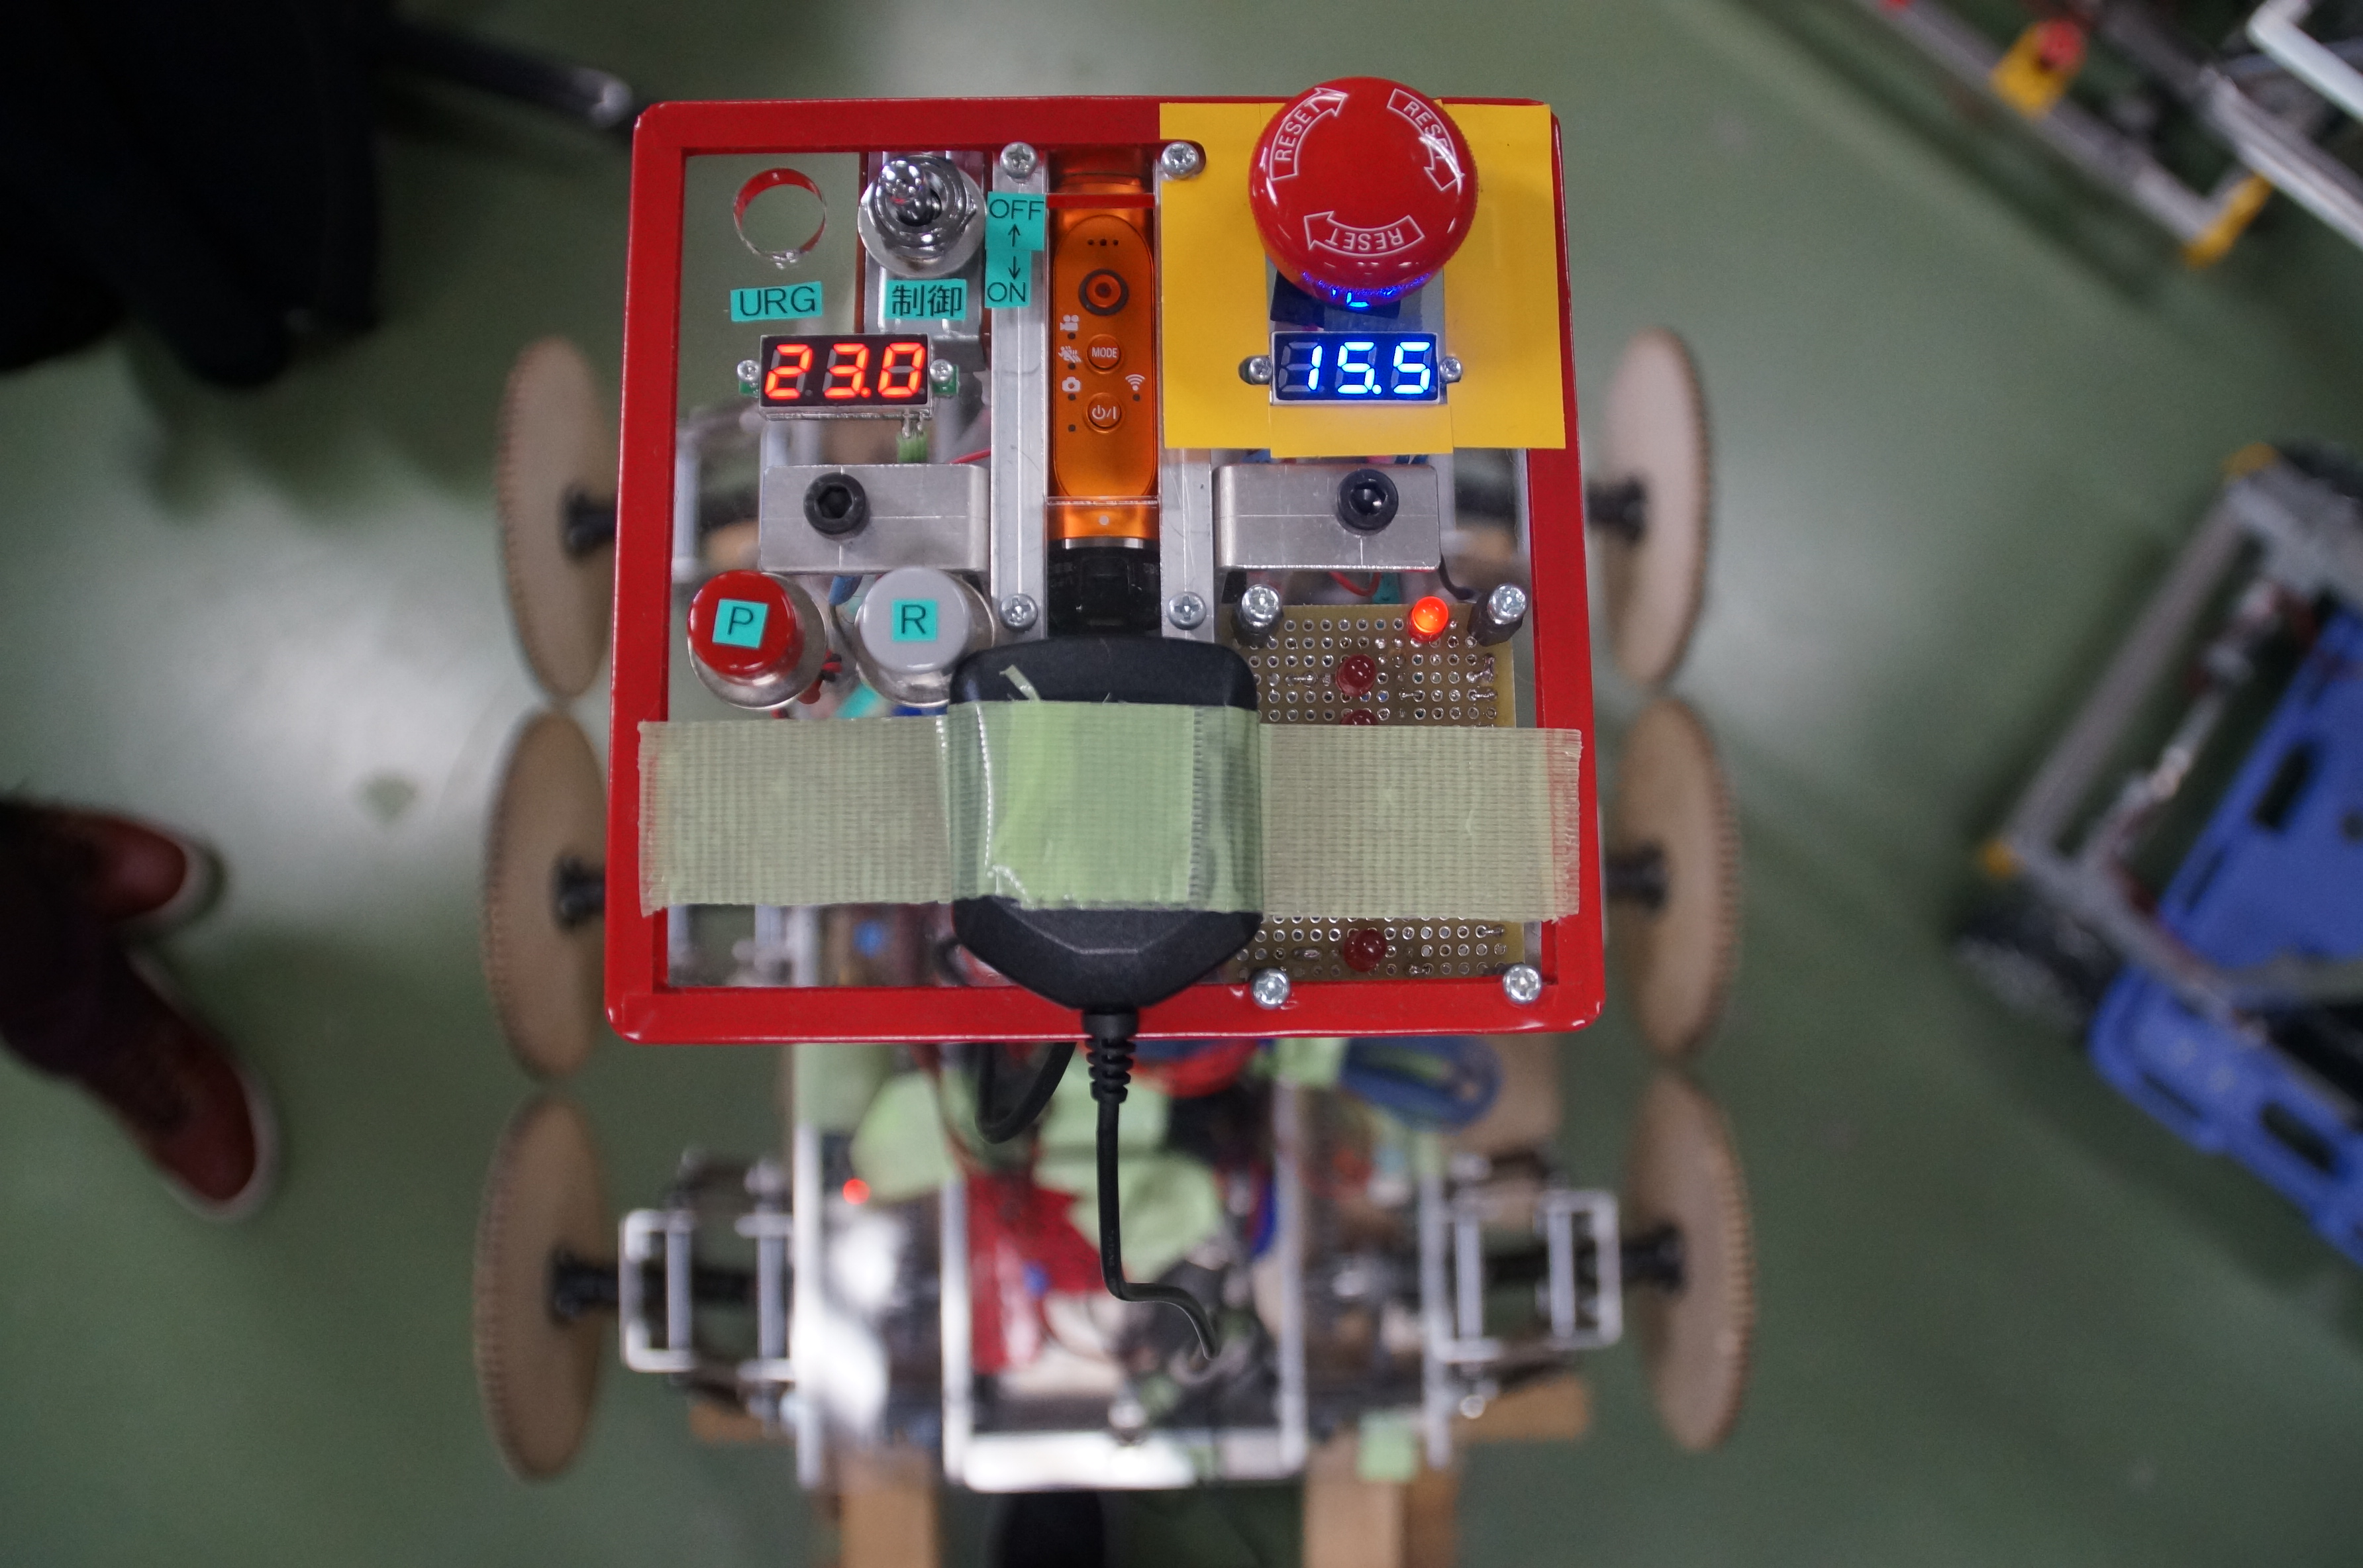
\includegraphics[width=80mm]{img/soft/DSC07946.jpg}
  \caption{操作パネル}
  \label{fig:start_panel}%ここに文章中で使用する名前を指定する
 \end{center}
\end{figure}

\subsection{無線通信}
\begin{enumerate}
\item 使用するデバイスをロボットが接続しているネットワークと同じネットワークに接続する.
\item sshコマンドを用いてロボットとデバイスを接続する.

(例 ssh ubuntu@192.168.2.116  ssh ユーザー名@ロボットのIPアドレス   
\item 接続が完了するとデバイス側のユーザー名がロボットのユーザー名に切り替わる.
\item 接続できない場合はロボットがネットワークに接続しているか確認する(ロボットのwifiドングルが機能しているかなど).  
\end{enumerate}



\mc
\section{機械の整備}
今回作成したロボットはパーツの点数が多く,持ち運ぶ際に分解した後の組み立てに時間がかかる.そこでロボットを駆動部である2つのDモジュールと中心部のCモジュールに分解させることで,最小限の分解で持ち運びを容易に行えるように設計した.これにより組み立ての時間を短縮することが狙いである
\subsection{必要な工具}
ロボットを分解,組み立てする際に必要な工具を以下に示す.基本的に全サイズを用意しておく.
\begin{enumerate}
 \item 六角レンチ
 \item レンチ
\end{enumerate}

\section{分解方法}
以下に分解手順を示す.本分解方法はつくばチャレンジ2016に参加した際に用いた方法と同様のものである.また,前提として上面のアクリル板に設置されたセンサ類のコードはすべて外してあり,別途に確保してある状態とする.
\begin{figure}[htp]
 \begin{center}
  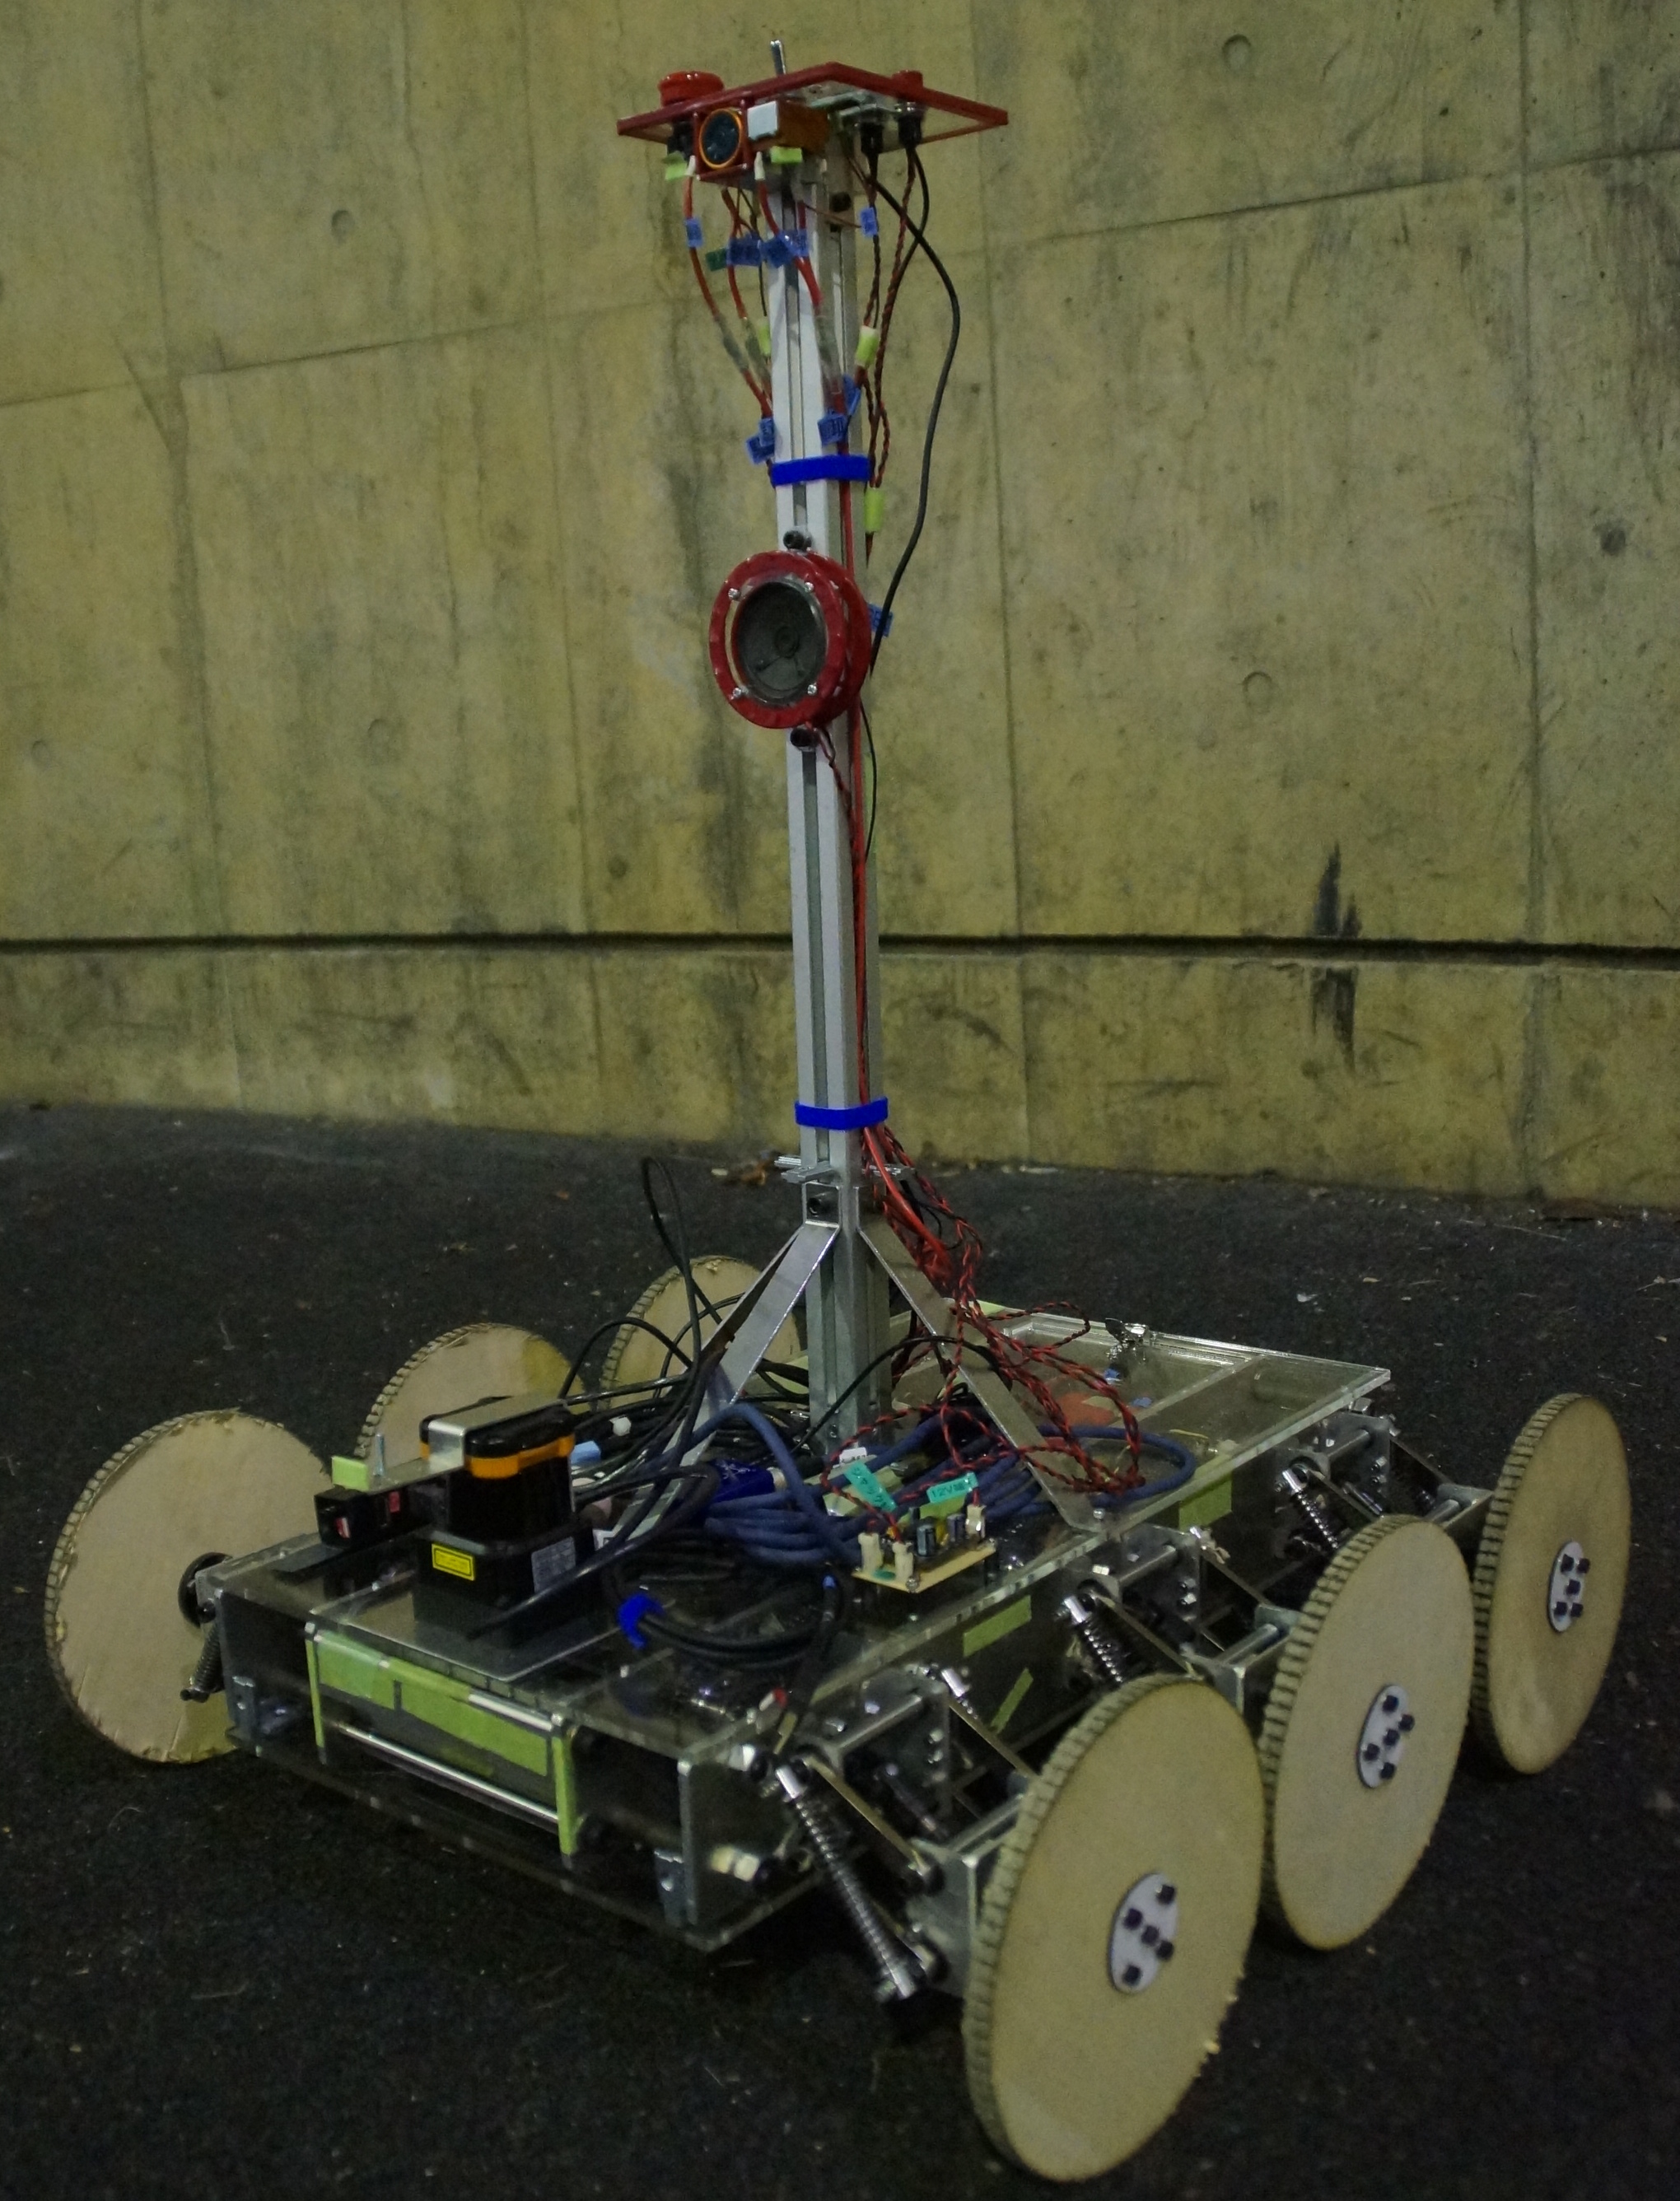
\includegraphics[width=80mm]{img/hard/zentai.jpg}
  \caption{ロボット図}
  \label{fig:robot}%ここに文章中で使用する名前を指定する
 \end{center}
\end{figure}

\subsection{ポールとアクリル板の取り外し}
ロボット上面のアクリル板はM3の六角穴付ボルトを使用している.ポールはM6の六角穴付ボルトとM3のボルトを使用している.

\begin{enumerate}
 \item アクリル板に取り付けてあるM3ボルトを全て取り外す.
 \item ポールのコード類が外されていることを確認し,アクリル板とポールを取り外す.(このときポールはアクリル板に固定されている状態である)
 \item ロボットをひっくり返し,腹面のアクリル板も同様に取り外す.
\end{enumerate}
なおポールそのものを持っての運搬,それに当たる行為は禁止である.アクリル板を落下し破損させる恐れがある.

\begin{figure}[htp]
 \begin{center}
  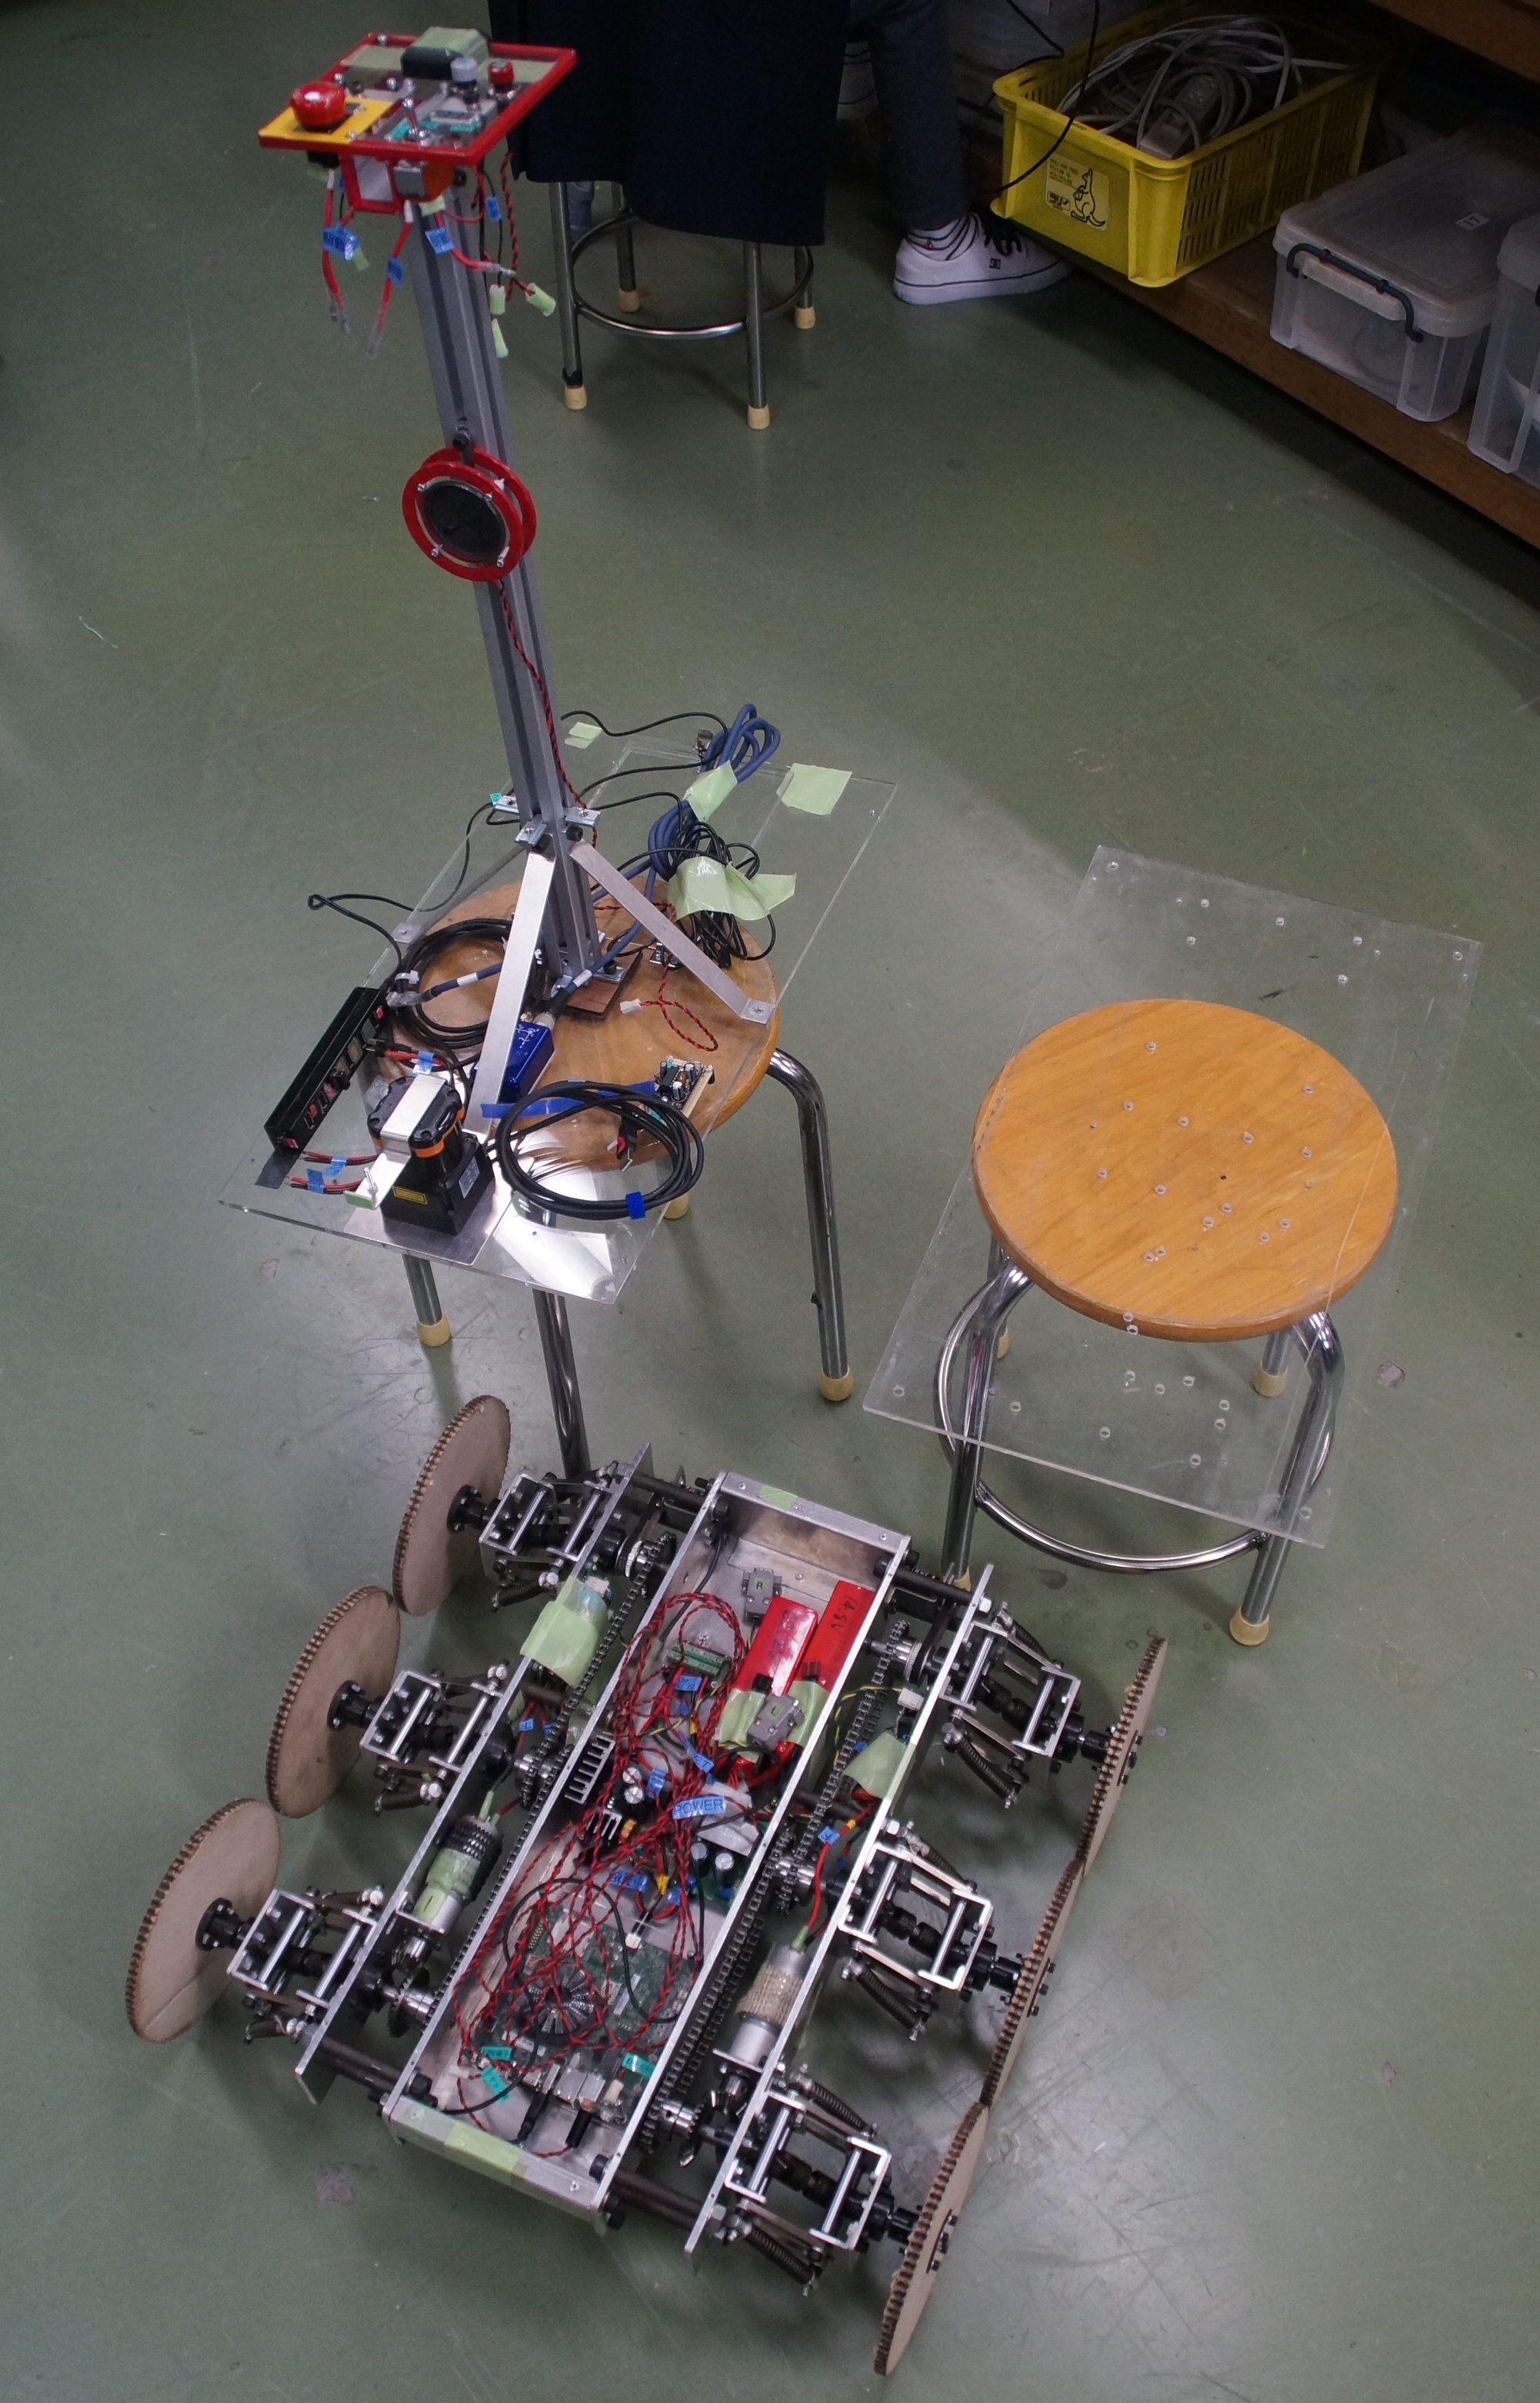
\includegraphics[width=80mm]{img/hard/f11.jpg}
  \caption{分解図}
  \label{fig:bunkai1}%ここに文章中で使用する名前を指定する
 \end{center}
\end{figure}



\subsection{DモジュールとCモジュールの分解}
この分解はDモジュールに接続されているコード類を引きちぎらないように注意を払って分解する.
ロボットの中心に保持されている部分がCモジュールである.CモジュールはM8の六角穴付ボルト4本で2つのDモジュールと接続されている
\begin{enumerate}
 \item M8ボルトを全て取り外し,Dモジュールを横に少し引き出す
 \item Dモジュールに接続されたシリアルケーブル(緑黄),電源ケーブル(赤黒),エンコーダケーブル(黒)を取り外す
 \item Dモジュールを完全に引き出し,Cモジュールを取り出す
\end{enumerate}
使用されているM8ボルトはDモジュールと一体化しているが問題はない,またカラーを無くさないようにする.くれぐれもコード類を引きちぎらないように注意する

\begin{figure}[htp]
 \begin{center}
  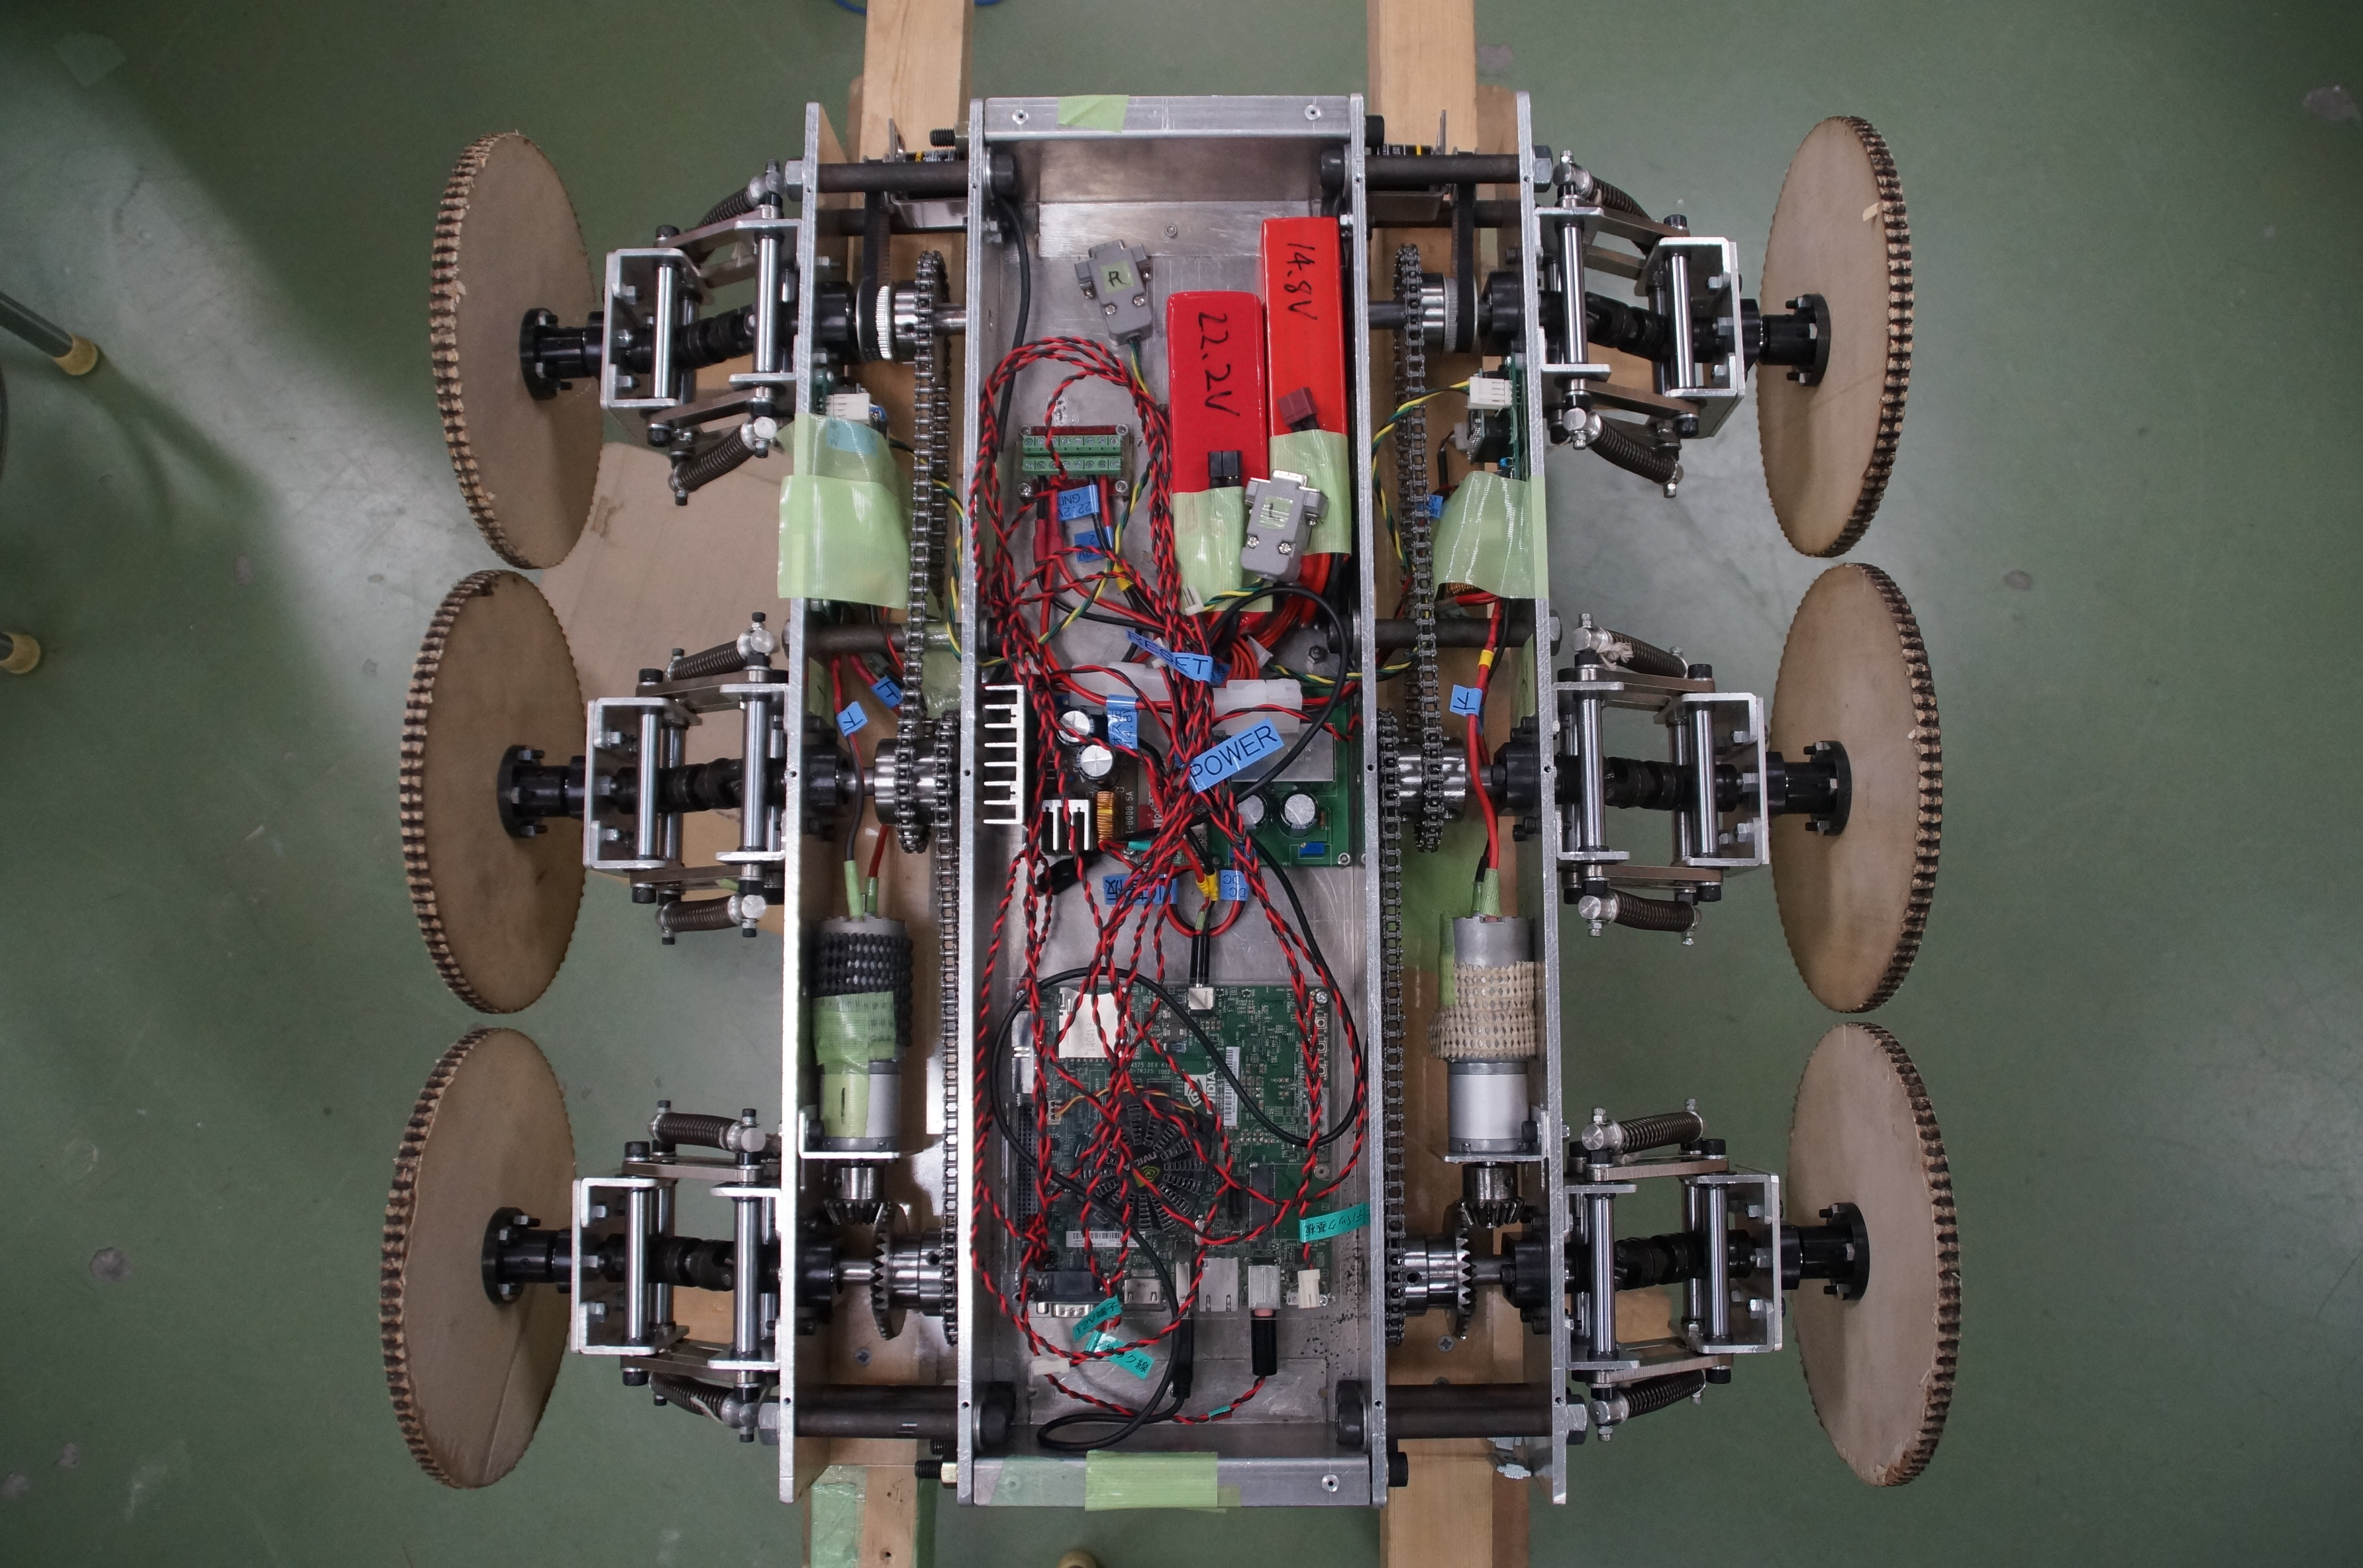
\includegraphics[width=80mm]{img/hard/f12.jpg}
  \caption{分解図}
  \label{fig:robot}%ここに文章中で使用する名前を指定する
 \end{center}
\end{figure}


\begin{figure}[htp]
 \begin{center}
  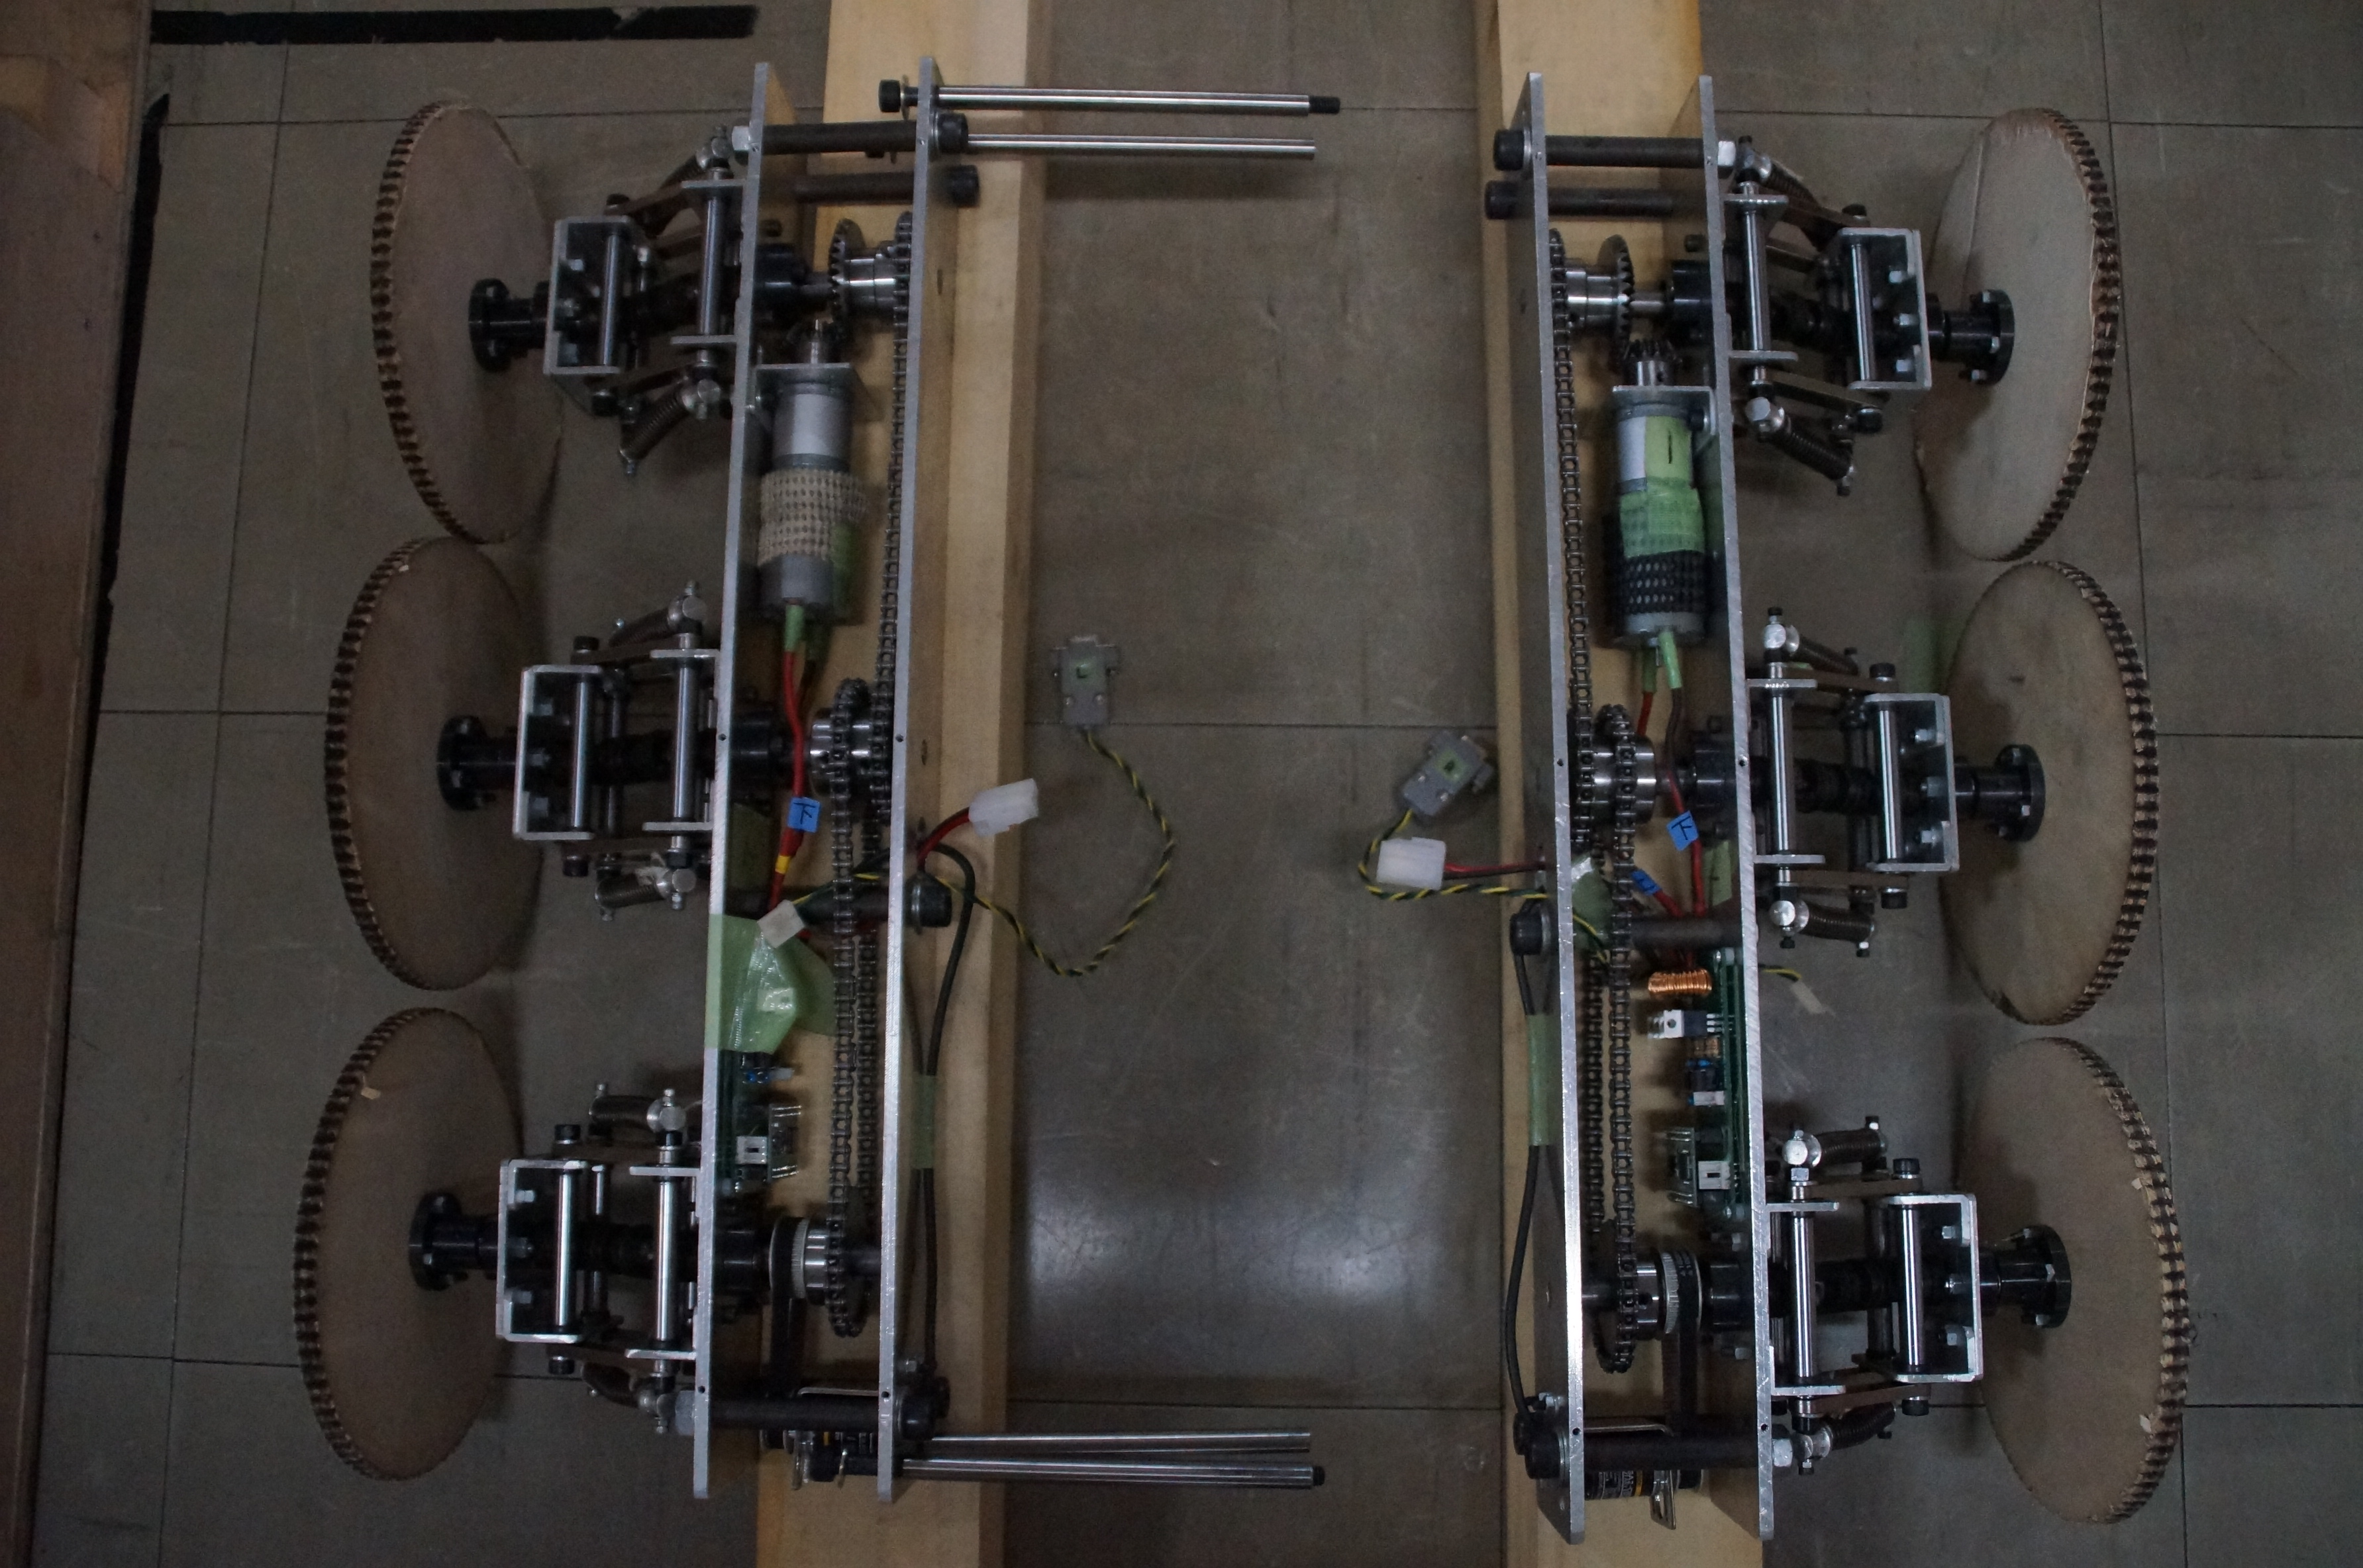
\includegraphics[width=80mm]{img/hard/f10.jpg}
  \caption{分解図}
  \label{fig:robot}%ここに文章中で使用する名前を指定する
 \end{center}
\end{figure}

\begin{figure}[htp]
 \begin{center}
  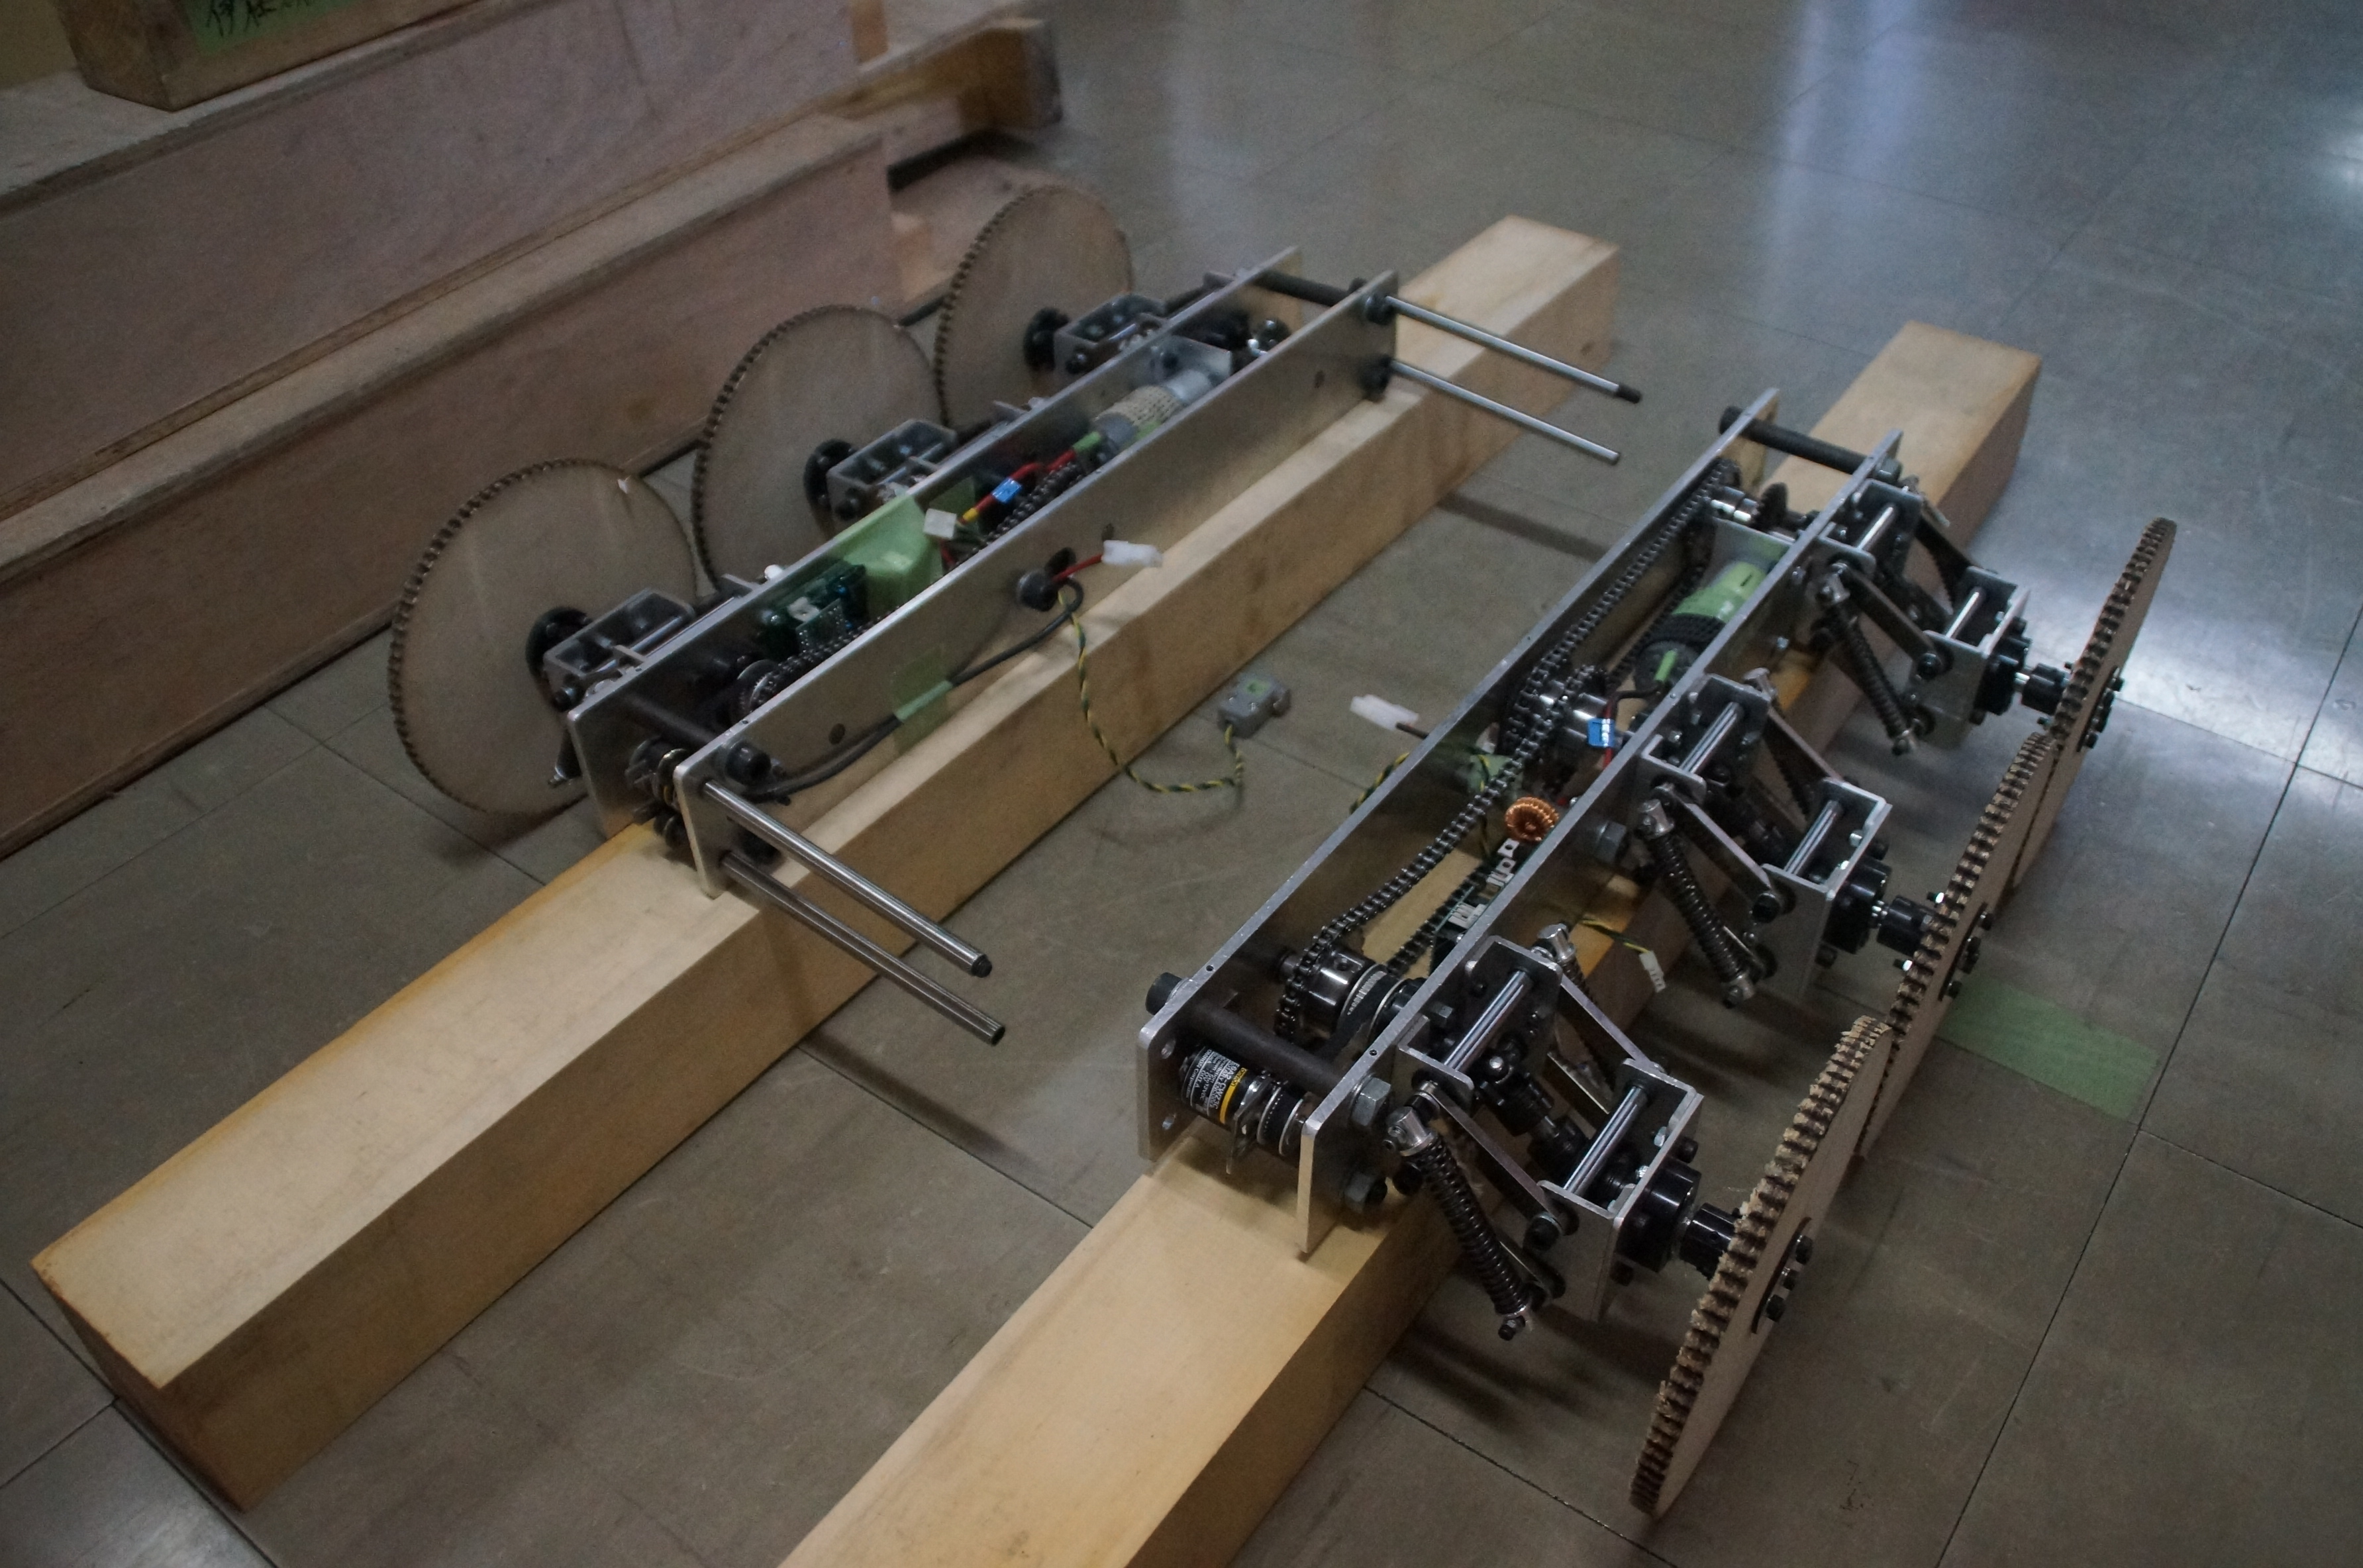
\includegraphics[width=80mm]{img/hard/f9.jpg}
  \caption{分解図}
  \label{fig:robot}%ここに文章中で使用する名前を指定する
 \end{center}
\end{figure}


\begin{figure}[htp]
 \begin{center}
  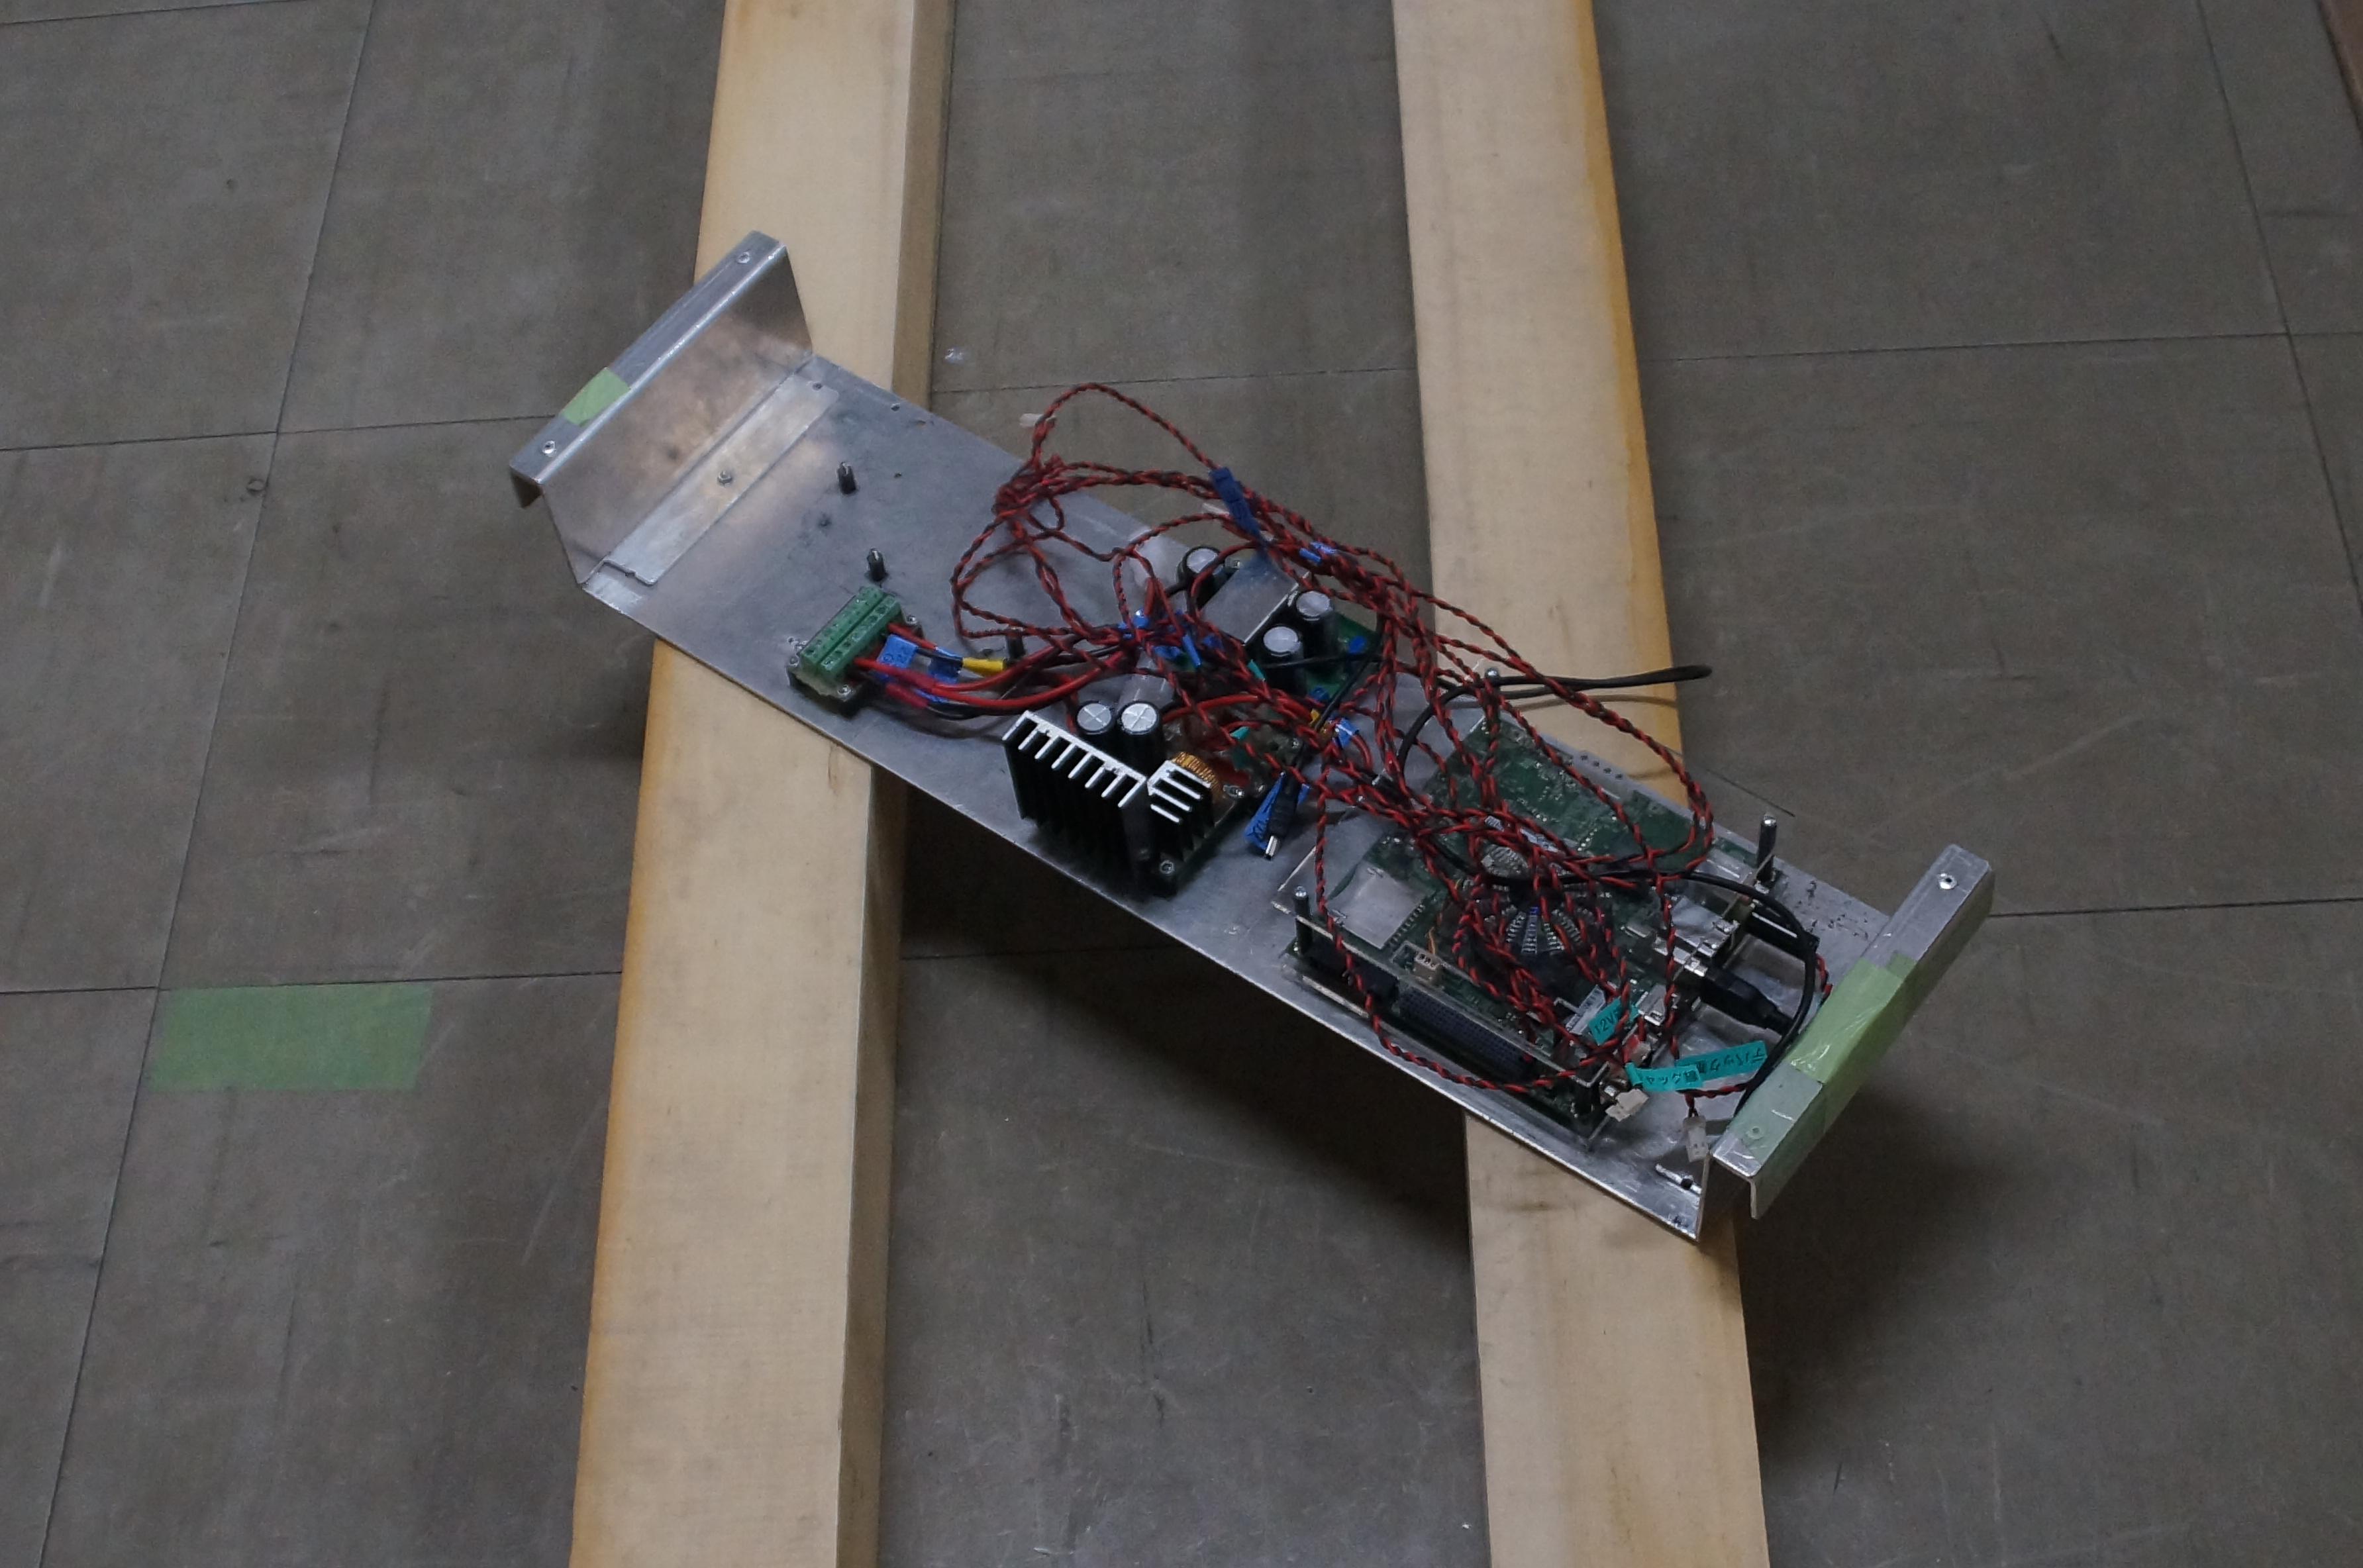
\includegraphics[width=80mm]{img/hard/f8.jpg}
  \caption{分解図}
  \label{fig:robot}%ここに文章中で使用する名前を指定する
 \end{center}
\end{figure}


\begin{figure}[htp]
 \begin{center}
  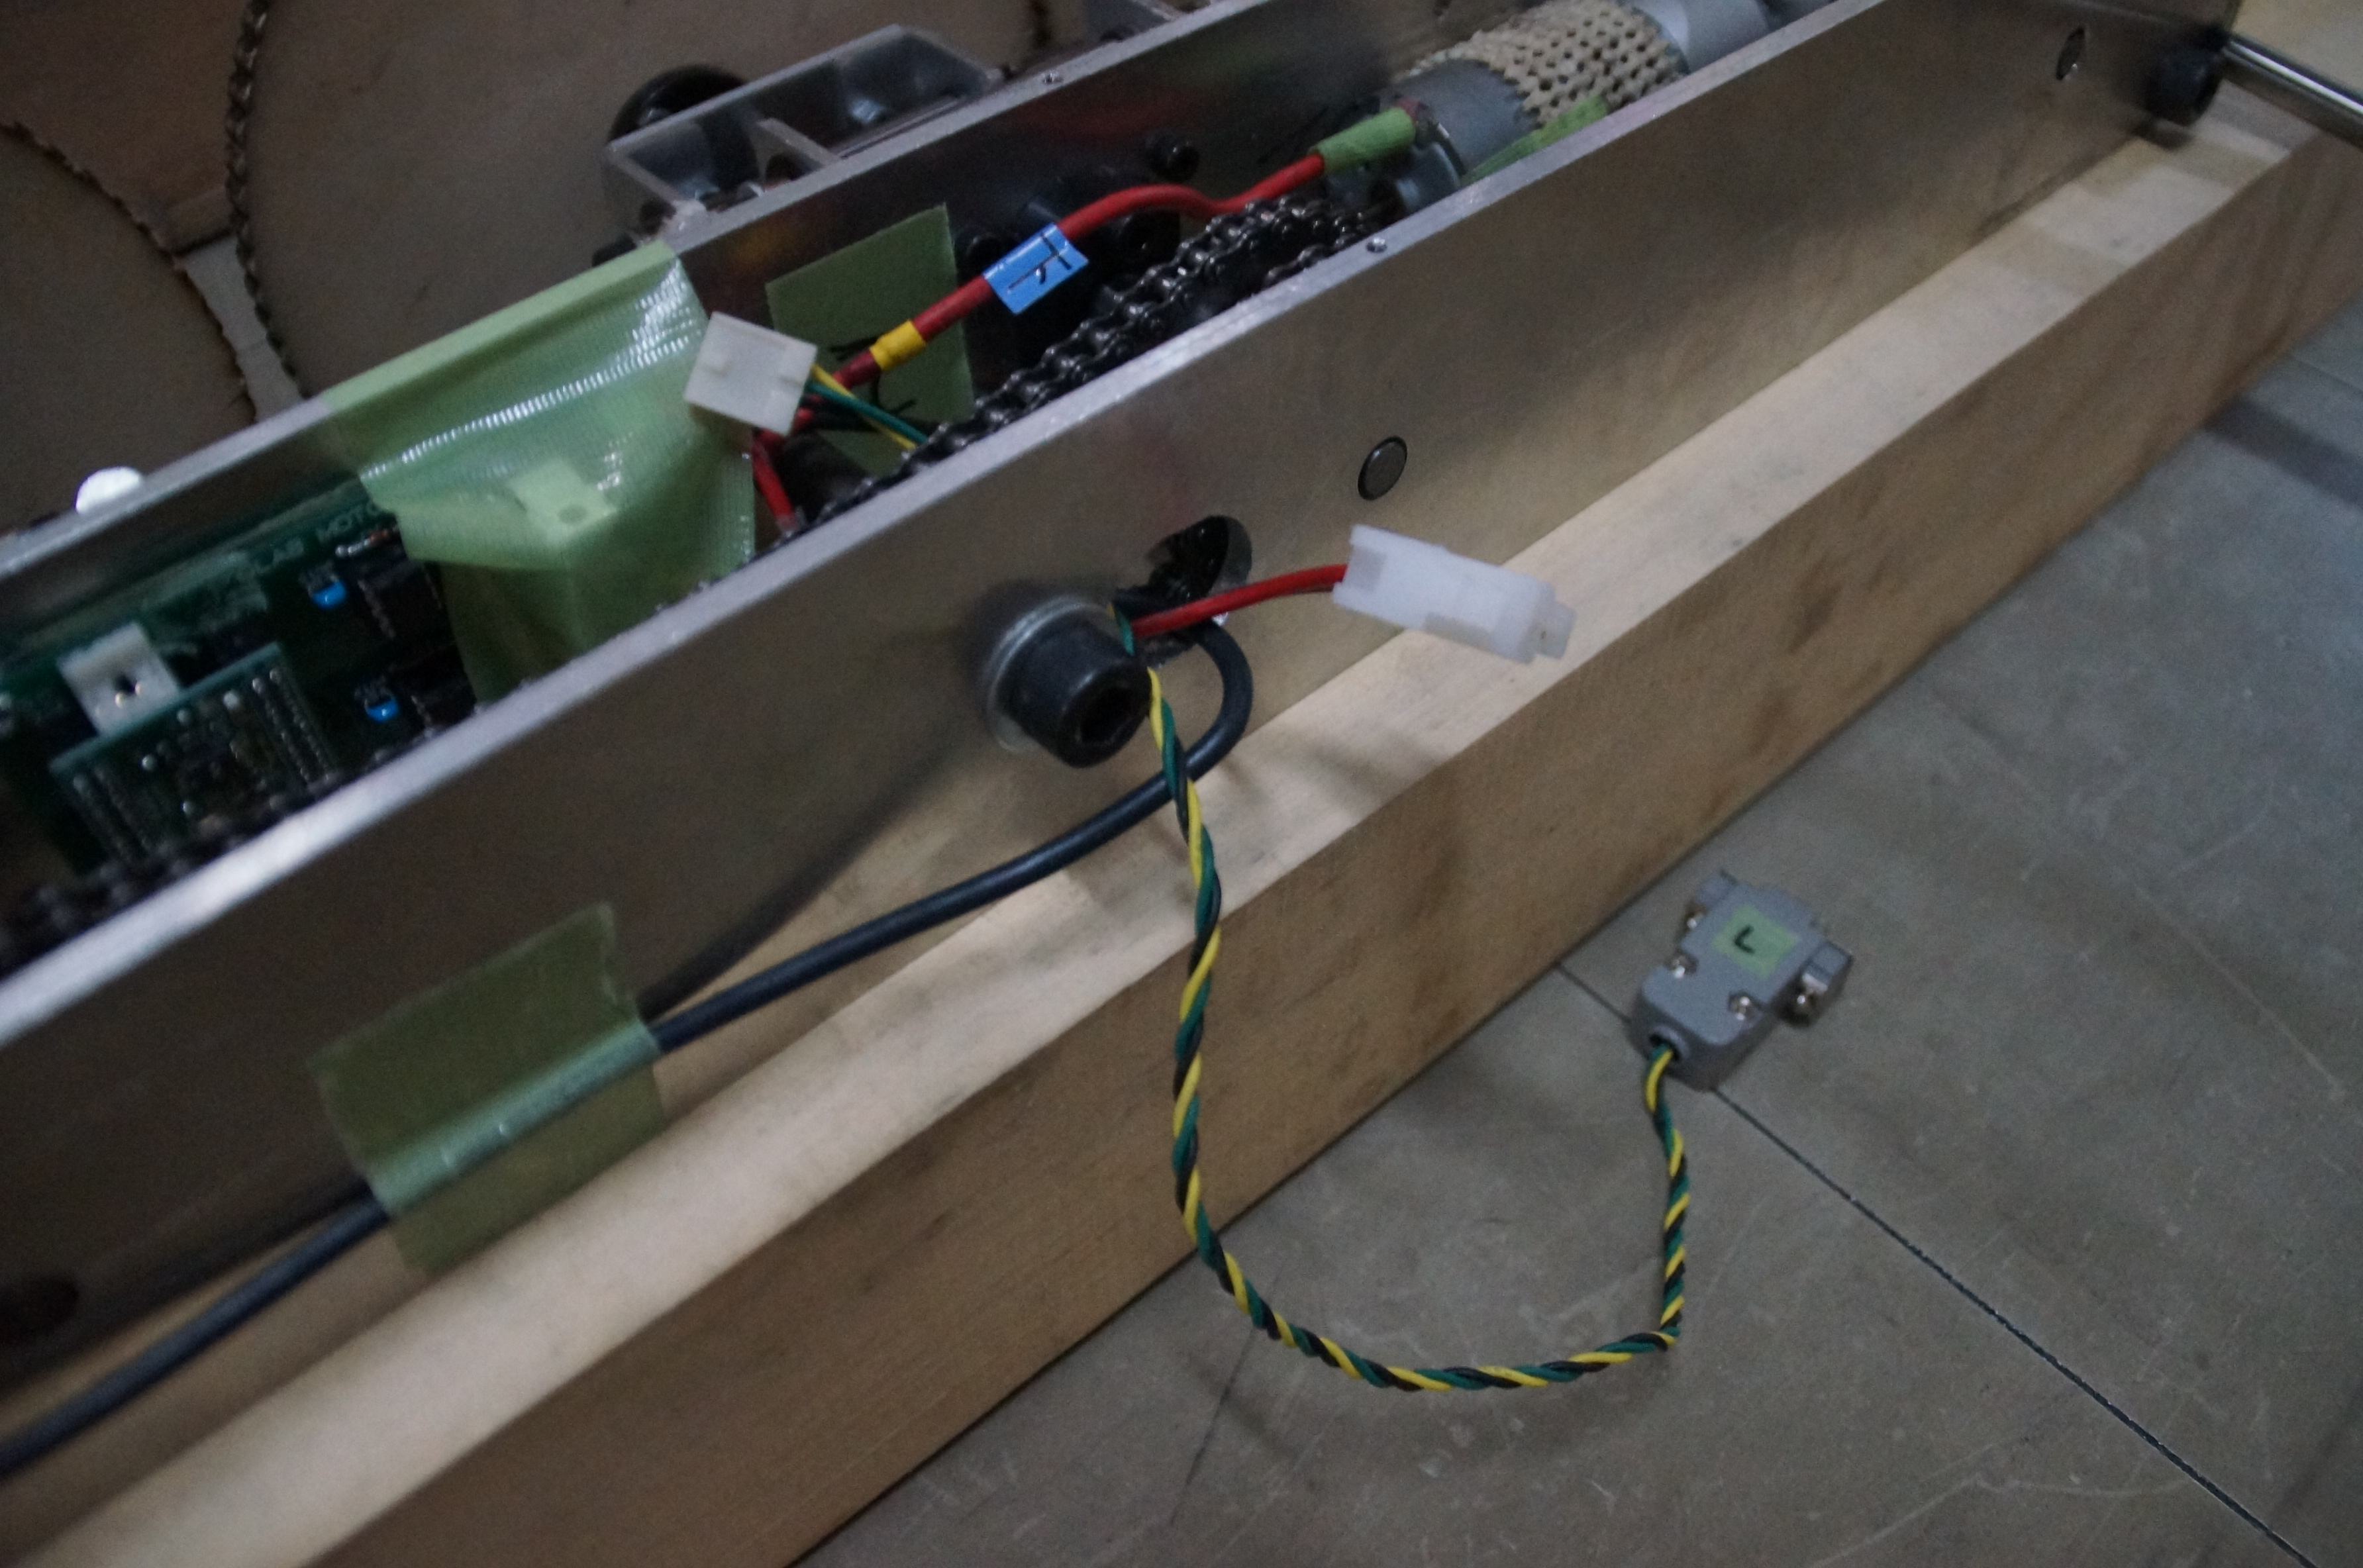
\includegraphics[width=80mm]{img/hard/f7.jpg}
  \caption{注意すべき配線}
  \label{fig:robot}%ここに文章中で使用する名前を指定する
 \end{center}
\end{figure}




\subsection{ポール分解}
ポールは支持パーツと操作パネル(カメラ内蔵)も接続されているため,それも分解する.ポールはM6のボルトを使用している.
\begin{enumerate}
 \item 底面に取り付けられている木の板を取り外し,支持パーツをスライドさせながら取り出す
 \item 操作パネルを保持するパーツを取り外し,操作パネルとポールを分離する 
 \item 操作パネルからカメラを取り外す
\end{enumerate}
支持パーツの中に1本だけ長いものがあるため,気をつけて整理する.
\begin{figure}[htp]
 \begin{center}
  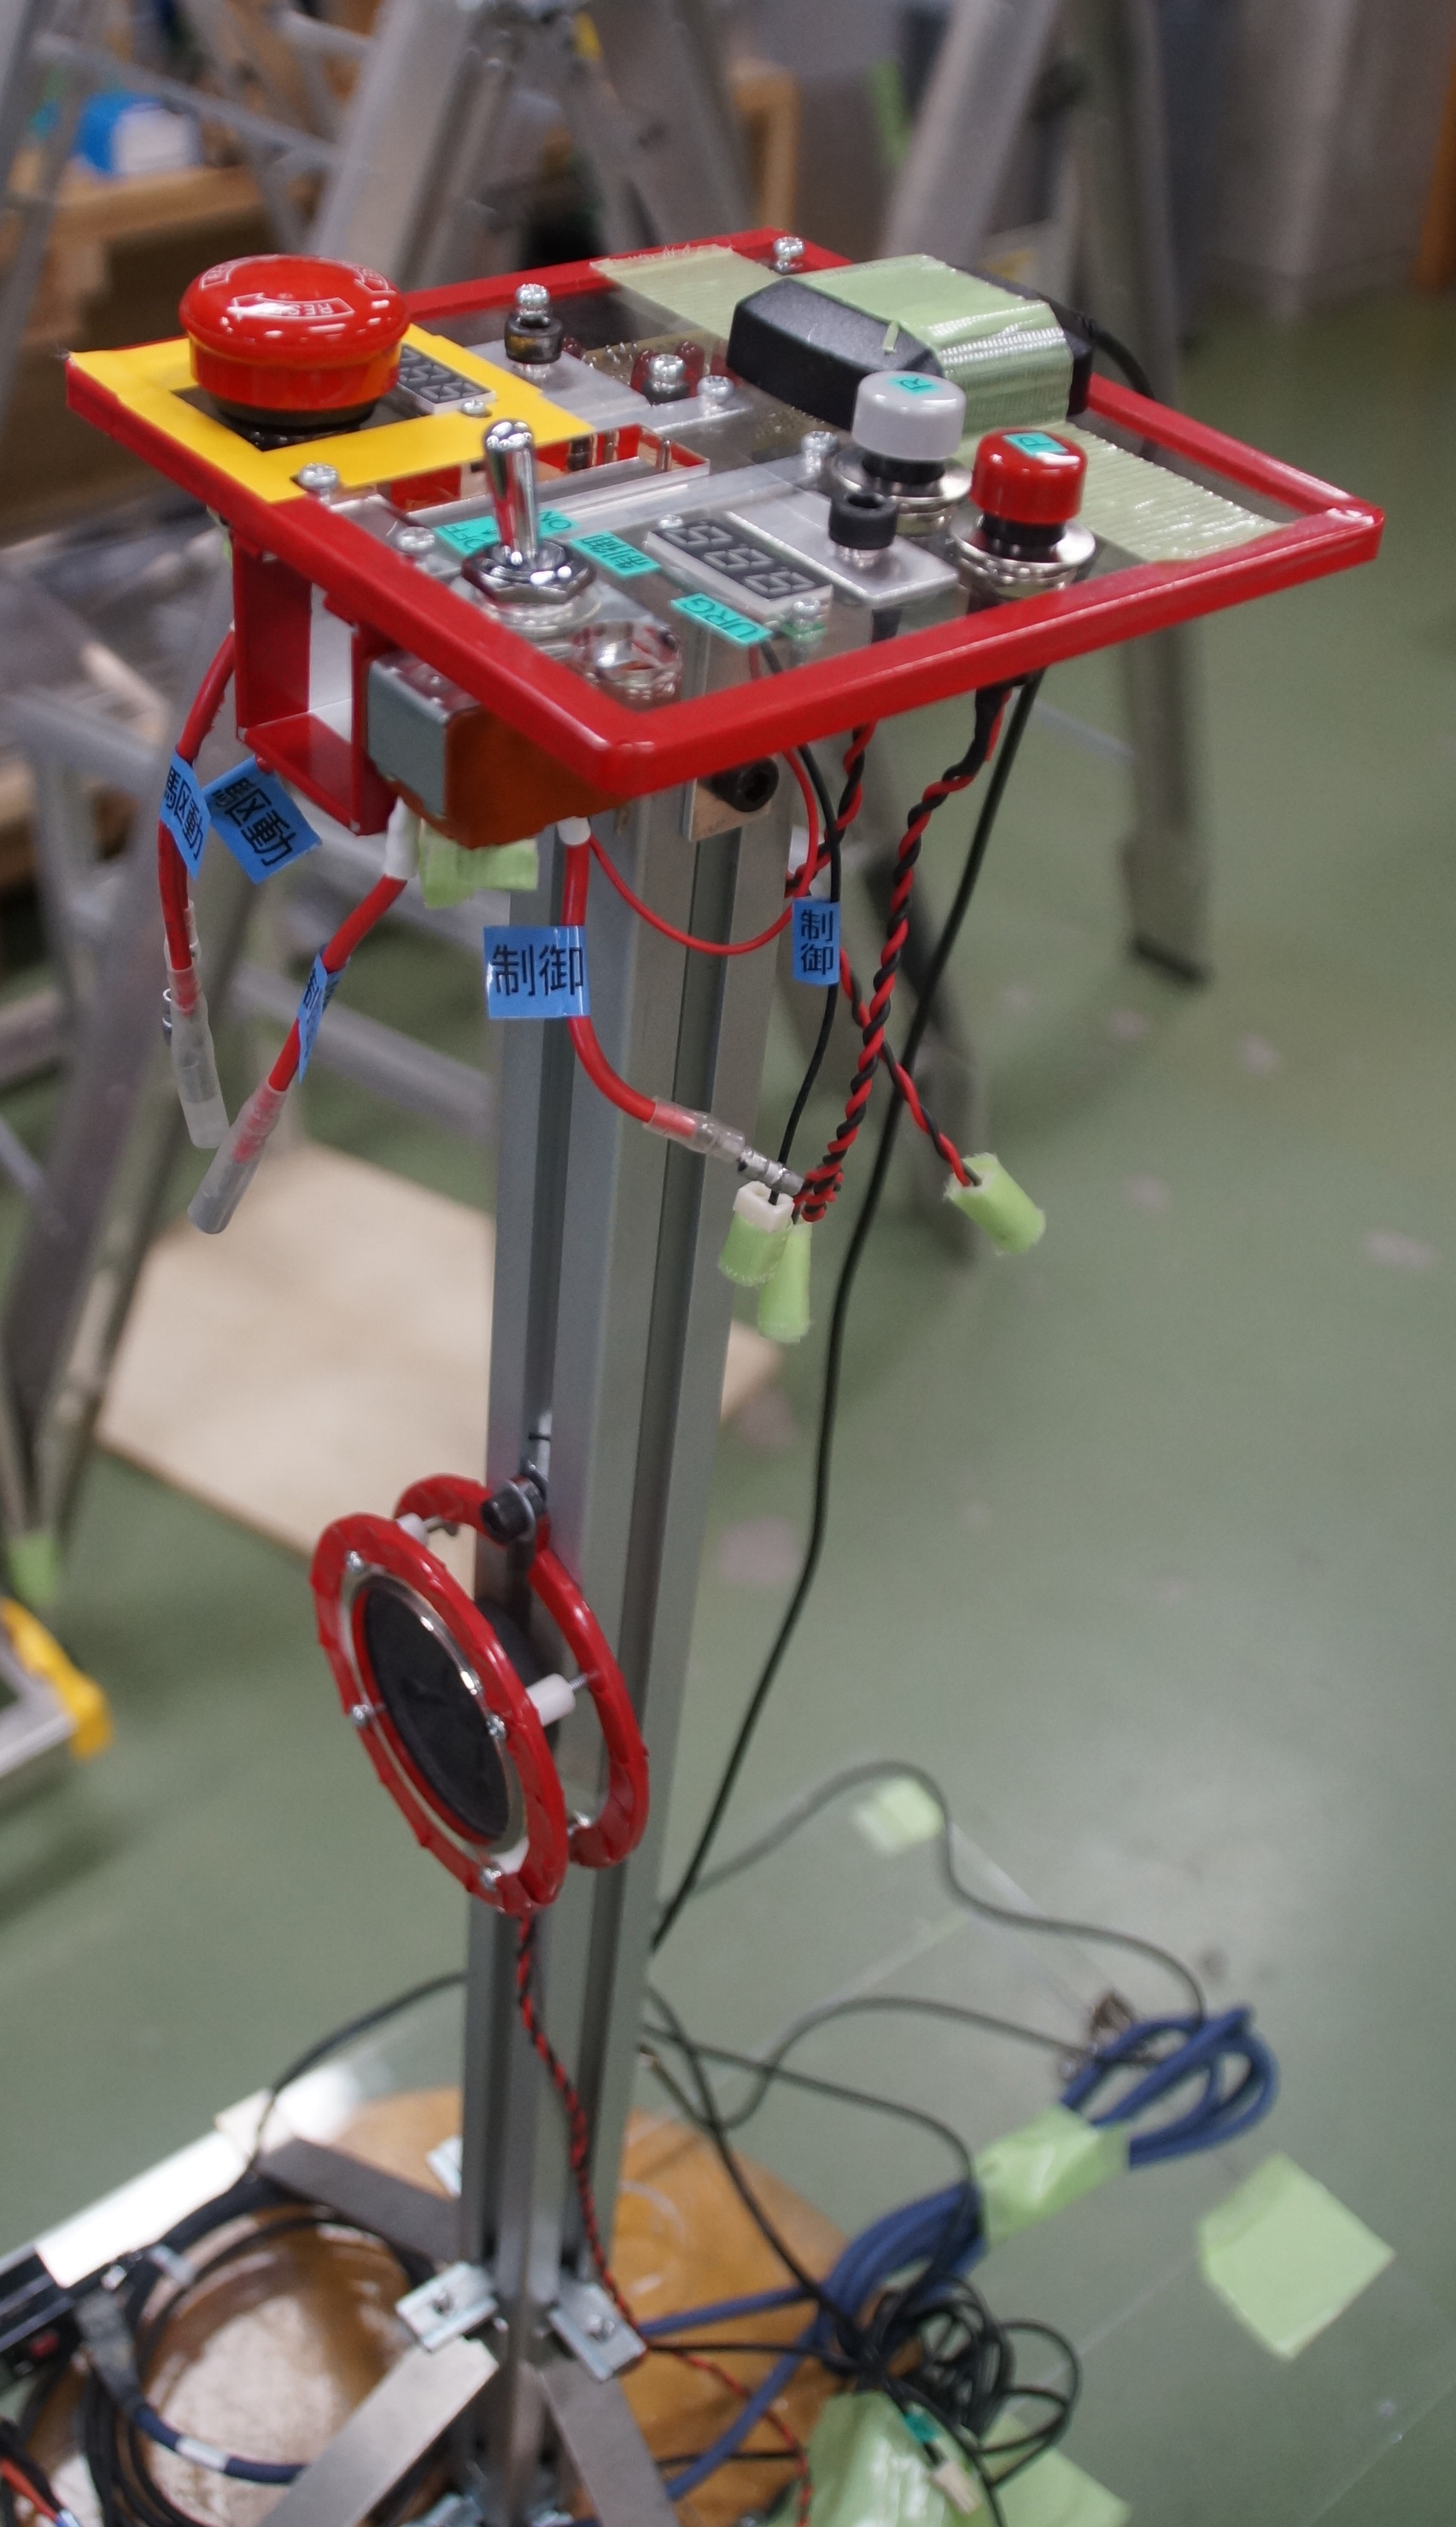
\includegraphics[width=80mm]{img/hard/f6.jpg}
  \caption{分解前}
  \label{fig:robot}%ここに文章中で使用する名前を指定する
 \end{center}
\end{figure}


\begin{figure}[htp]
 \begin{center}
  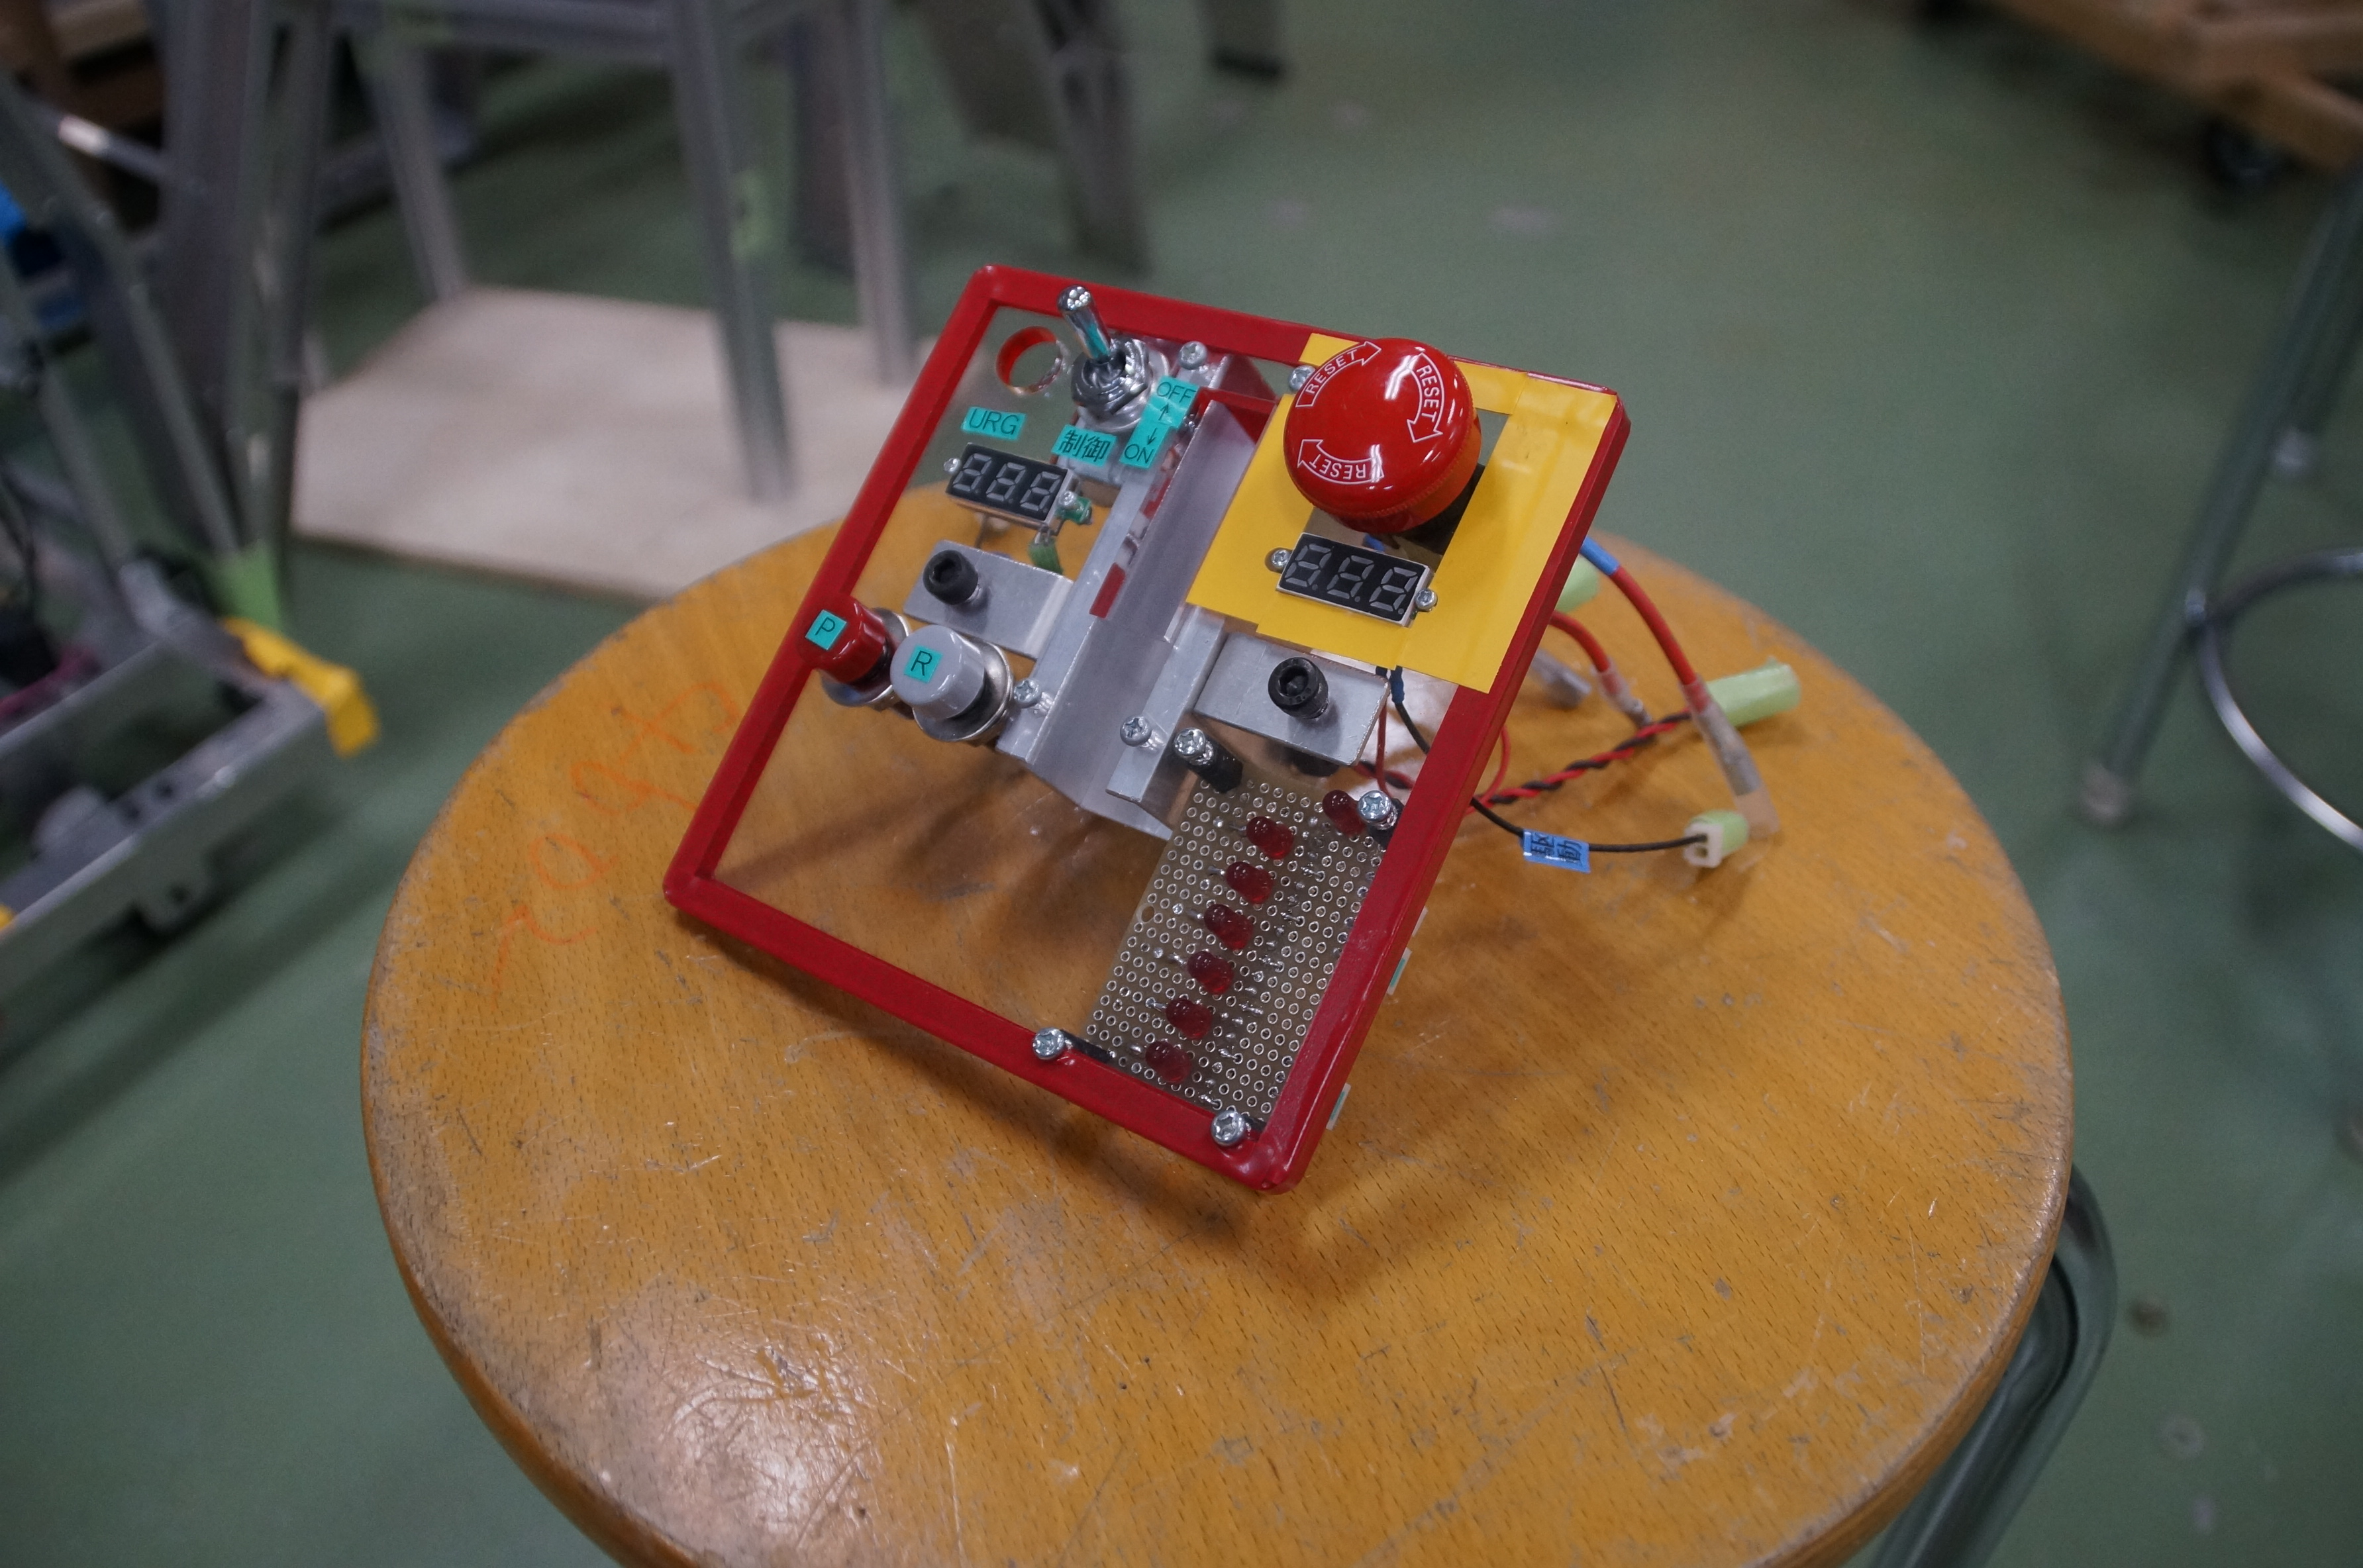
\includegraphics[width=80mm]{img/hard/f5.jpg}
  \caption{分解図}
  \label{fig:robot}%ここに文章中で使用する名前を指定する
 \end{center}
\end{figure}
\subsection{センサの取り外し}
上面アクリル板はモーションセンサと測域センサを取り付けてあるため,これも外し個包装を施す.

\subsection{箱つめ}
分解したD,Cモジュールを箱に詰める.詰める際にはCモジュールに接続されたセンサ関連は全て取り外し保管する.


\end{document}



